\documentclass[a4paper]{llncs}

\usepackage{amsmath}
\usepackage{xspace}
\usepackage{booktabs}
\usepackage{relsize}
\usepackage{multirow}
\usepackage{derriclst}
\usepackage[scaled=0.8]{beramono}
\usepackage[T1]{fontenc}
\usepackage{url}
\usepackage{boxedminipage}
\usepackage{tikz}
\usepackage{array}
\usepackage{pgfplots}
\usepackage{mathptm}
\usepackage{stmaryrd}

\def\derric{\textsc{Derric}\xspace}

\newcommand{\JPEG}{\textsmaller{JPEG}\xspace}
\newcommand{\GIF}{\textsmaller{GIF}\xspace}
\newcommand{\PNG}{\textsmaller{PNG}\xspace}
\newcommand{\GB}{\textsmaller{GB}\xspace}
\newcommand{\DSL}{\textsmaller{DSL}\xspace}
\newcommand{\EXIF}{\textsmaller{EXIF}\xspace}

\def\mykeyword#1{\textbf{\texttt{#1}}}
\def\identifier#1{\texttt{#1}}

\def\levelGood{\ensuremath{Low}\xspace}
\def\levelOk{\ensuremath{Medium}\xspace}
\def\levelBad{\ensuremath{High}\xspace}

\begin{document}

\title{A Case Study in Evidence-Based DSL Evolution}

\author{Jeroen van den Bos\inst{1,2} \and Tijs van der Storm\inst{1}}
\institute{Centrum Wiskunde \& Informatica, Amsterdam, The Netherlands
\and Netherlands Forensic Institute, Den Haag, The Netherlands\\
\email{jeroen@infuse.org}, \email{storm@cwi.nl}}

\maketitle

\begin{abstract}
Domain-specific languages (\DSL{}s) can significantly increase productivity and quality in software construction. 
However, even \DSL programs need to evolve to accomodate changing requirements and circumstances.
How can we know if the design of a \DSL supports the relevant evolution scenarios on its programs?
We present an experimental approach to evaluate the evolutionary capabilities of a \DSL and apply it on a \DSL for digital forensics, called \derric.
Our results indicate that the majority of required changes to \derric programs are easily expressed.
However, some scenarios suggest that the \DSL design can be improved to prevent future maintenance problems.
Our experimental approach can be considered first steps towards evidence-based \DSL evolution.
\end{abstract}

\section{Introduction\label{sect:introduction}}

\noindent
Domain-specific languages (\DSL{}s) can increase productivity by trading generality for expressive power~\cite{MernikEtAl05,vanDeursenEtAl00}.
Furthermore, \DSL{}s have the potential to improve the practice of software maintenance: routine changes are easily expressed. 
More substantial changes, however, might require the \DSL itself to be changed~\cite{vanDeursenKlint98}. 
How can we find out whether the relevant maintenance scenarios will require routine changes or not?

In this paper we present a test-based experimental approach to answer this question and apply it to a domain-specific language for describing file formats: \derric~\cite{derric_casestudy}.
\derric is used in the domain of digital forensics to generate software to analyze, reconstruct, and recover file-based evidence from storage devices.
In digital forensics it is common that such file format descriptions need to be changed regularly, either to accomodate new file format versions, or to deal with vendor idiosyncrasies. 

As a starting point, we have assembled a large corpus of image files to trigger failing executions of the file recognition code that is generated from \derric descriptions.
Each failing execution is attempted to be corrected through a modification of the \derric code, until all image files are correctly recognized.
The required changes are accurately tracked, categorized and rated in terms of complexity.
This set of changes provides an empirical baseline to assess whether the design of \derric sufficiently facilitates necessary maintenance.

The results show that all of the required changes were expressible in \derric; the \DSL did not have to be changed to resolve all failures.
The majority of harvested changes consists of multiple, inter-dependent modifications. 
The second most common change consists of a single, simple, local modification.
Finally, a minority of changes is more complex.
We discuss how the \derric \DSL may be changed to make these changes expressed more easily.
Thus, the experiment has provided us with empirical data to improve the design of \derric.

The contributions of this paper can be summarized as follows:
\begin{itemize}
\item We describe and apply an experiment in \DSL-based maintenance in the context of \derric, and provide a detailed description including its parameters.
\item We present empirical results on how the \derric \DSL supports the maintenance process in the domain of digital forensics.
\item We discuss the usefulness of this approach and how it has helped us to both evaluate and improve the design of \derric.
\end{itemize}
These contributions can be considered first steps towards evidence-based \DSL evolution. 

\section{Background\label{sect:background}}

\noindent
\derric is a \DSL to describe binary file formats~\cite{derric_casestudy}. 
It is used in digital forensics investigations to construct highly flexible and high performance analysis tools. 
One example is the construction of file carvers~\cite{derric_background}, which are used to recover possibly damaged evidence from confiscated storage devices (e.g., hard disks, cameras, mobile phones etc.). 
\derric descriptions are used to generate some of the software components, called \textit{validators}, that check whether a recovered piece of data is a valid file of a certain type.

\begin{figure}[t]
\begin{multicols}{2}
\begin{lstlisting}[language=derric, numbers=left, numberstyle=\tiny, numbersep=1pt]
format PNG
extension png
strings ascii
sequence Signature IHDR Chunk* IEND

structures
Signature {
    marker: 137,80,78,71,13,10,26,10; 
}

Chunk {
  length: lengthOf(chunkdata) size 4;
  chunktype: type string size 4;
  chunkdata: size length;
  crc: checksum(
         algorithm="crc32-ieee",
         init="allone",start="lsb",
         end="invert",store="msbfirst",
         fields=chunktype+chunkdata)
       size 4; 
}

IHDR = Chunk {
  chunktype: "IHDR";
  chunkdata: {
    width: !0 size 4;
    height: !0 size 4;
    bitdepth: 1|2|4|8|16;
    colourtype: 0|2|3|4|6;
    compression: 0;
    filter: 0;
    interlace: 0|1;
  }
}

IEND {
  length: 0 size 4;
  chunktype: "IEND";
  crc: 0xAE,0x42,0x60,0x82;
}
\end{lstlisting}
\end{multicols}


\caption{Simplified \PNG in \derric.\label{FIG:png}}
\end{figure}

An example \derric description for a simplified version of the \PNG file format is shown in Fig.~\ref{FIG:png}.
The structure of a file format is declared using the \mykeyword{sequence} keyword. 
The sequence consists of a regular expression that specifies the syntax of a file format in terms of basic blocks, called \textit{structures}. 
In this case, a \PNG file starts with a \identifier{Signature} block, an \identifier{IHDR} block, zero-or-more \identifier{Chunk}s and finally an \identifier{IEND} block. 

The contents of each structure is defined in the following \mykeyword{structures} section.
A structure consists of one or more fields. 
The contents and size of each field are constrained by expressions. 
The simplest expression is a constant, that directly specifies the content, and hence length, of a field.
This is the case for the \identifier{marker} field of the \identifier{Signature} structure.
Another common type of constraint only restricts the type and/or length of a field.
For instance, the \identifier{chunktype} field of structure \identifier{Chunk} is constrained to be of type \identifier{string} and size 4.
Constraints may involve arbitrary content analyses.
For example, consider the \identifier{crc} field. 
To recognize this field a full checksum analysis following the \texttt{crc32-ieee} algorithm should be performed. 

\section{Observing Corrective Maintenance\label{sect:approach}}

\noindent
To study the maintainability characteristics of \derric, we need a way to inspect and evaluate actual maintenance scenarios. 
In other words: we need to observe how \DSL programs are changed.
For the purpose of this paper, we focus on \textit{corrective} maintenance~\cite{ISO14764}, which is maintenance in response to observed failures (``bug fixing''). 

To realize this, a large corpus of representative and relevant inputs to a \DSL program is needed, which allows us to automatically generate failures, which in turn trigger corrective maintenance actions.
The approach is similar to \textit{fuzzing} where a program is run on large quantities of invalid, unexpected or even random input data~\cite{Oehlert05}. 
For maintenance evaluation, however, it is of paramount importance that the data is representative of what would be encountered in practice.

In the case of \derric we have assembled a large, representative corpus of image files (\JPEG, \GIF and \PNG) for which \derric descriptions are available. 
The exact nature of these descriptions and the corpus is described in detail in Section~\ref{sect:experiment}.

For each file format $f$, the initial \derric $D^i_f$ description is compiled to a validator and subsequently run on the corpus files of type $f$.
This results in an initial set of files for which validation fails\footnote{Technically, both false positives and false negatives are failures. However, since the corpus only contains real files, we cannot detect when a validator would incorrectly validate a file.}.
The set of failures is then divided over equivalence classes which are sorted by their size.
This allows us to focus on the most urgent problems first.
Next, $D^i_f$ is edited to obtain a new version $D^{i+1}_f$ which resolves at least one of the failures in the largest equivalence class. 
As soon as the set of failures is observed to decrease, $D^{i+1}_f$ is committed to the version control system.
Before committing we ensure that the set of correctly validated files (the true positives) strictly increases, as a form of regression test.
The process then repeats, now using $D^{i+1}_f$ as a starting point.

After all failures have been resolved, the changes, as stored in the version control, are categorized in \textit{change complexity classes}. 
A change may thus be interpreted as being more complex than another change. 
This provides an empirical base line to qualitatively assess to what extent \derric supports maintenance of format descriptions. 

\section{Experiment\label{sect:experiment}}

\subsection{\DSL Programs and Corpus\label{sect:corpus}}

\noindent
The three \DSL programs that have been used are \derric descriptions of \JPEG, \GIF and \PNG.
These file formats are well-known, very common and highly relevant to the practice of digital forensics. 
An impression of the sizes of these descriptions is given in Table~\ref{tab:initial}. 
From the table it can be inferred that the descriptions are significantly different.
Both \GIF and \PNG have a richer syntactic structure than \JPEG. 
Structure inheritance is heavily used in  \JPEG and \PNG but only once in \GIF. 
Finally, \GIF has a lot more fields per structure (58 per 12). 
Summarizing, we claim that the three file format descriptions cover a wide range of \derric's language features, in different ways.

\begin{table}[h]\centering
\begin{minipage}{.49\textwidth}\centering
\vspace{13pt}
\begin{tabular}{lrrr}
& \multicolumn{1}{c}{\JPEG} & \multicolumn{1}{c}{\GIF} & \multicolumn{1}{c}{\PNG} \\
\midrule
Sequence tokens & 14 & 29 & 30 \\
Structures & 15 & 12 & 20 \\
Uses of inheritance & 10 & 1 & 17 \\
Field definitions & 32 & 58 & 27 \\
\midrule
\end{tabular}
\vspace{5pt}
\caption{Initial \derric descriptions.\label{tab:initial}}
\end{minipage}
\begin{minipage}{.49\textwidth}\centering
\begin{tabular}{crrrr}
& \multicolumn{2}{c}{Data Set} &
\multicolumn{2}{c}{Failures}\\
\multicolumn{1}{c}{Format} &
\multicolumn{1}{c}{\#} & \multicolumn{1}{c}{size} &
\multicolumn{1}{c}{\#} & \multicolumn{1}{c}{\%}\\
\midrule
\JPEG &
930,386 & 327\GB &
5,485 & 0.6\% \\
\GIF &
36,524 & 3\GB &
389 & 1.1\% \\
\PNG &
236,398 & 27\GB &
5,789 & 2.4\% \\
\midrule
Total & 1,203,308 & 357\GB &
11,663 & 1.0\% \\
\end{tabular}
\vspace{5pt}
\caption{Initial validator results.\label{TAB:initial}}
\end{minipage}
\end{table}

The second important component of the experiment, is a representative corpus. 
We have developed such a corpus for the evaluation of our earlier work on model-transformation of \derric descriptions~\cite{derric_transformations}. 
This data set contains \JPEG, \GIF and \PNG images found on Wikipedia, downloaded using the latest available static dump list, which dates from 2008\footnote{Available at \url{https://github.com/jvdb/derric-eval}}.
Around 50\% of the files on that list were still available and included in the set.
An overview of the data set is shown in Table~\ref{TAB:initial}. 
The corpus contains a total of 1,203,410 images, leading to a total size of 357 \GB. 
As the last two columns show, not all images in the data set are recognized by the validators generated from the respective \JPEG, \GIF and \PNG descriptions: between 0.6\% and 2.4\% of the files in the data set are not recognized using the base descriptions of the respective file formats.

The Wikipedia data set can be considered representative, since the files uploaded to it originate from many different sources (e.g., cameras, editing software, etc.).
We have verified this diversity by inspecting the metadata of the files and aggregating the results.

This shows that the set contains files from a large number of different cameras (e.g., Canon, Nikon, etc.)
Furthermore, many images have been modified using a multiplicity of tools (e.g., Photoshop, Gimp, etc.)
Original computer images such as diagrams and logos have been created using many different tools (e.g., Dot, Paintshop Pro, etc.)

The diversity is depicted graphically in Fig.~\ref{fig:software}, showing the distribution of files over values of the \EXIF \textit{Software} tag present in 28.4\% of the images.
The most common tool is Photoshop 7.0, used on 3.4\% of the corpus; Photoshop CS2 and CS (Windows) are used on 2.3\% and 1.8\% respectively.
ImageReady covers 1.6\%.
After that the percentages rapidly decrease:
no specific version of any application was used in more than 1\% of the files. 
The number of different values is 4,024.

\begin{figure}
\begin{center}
{\small
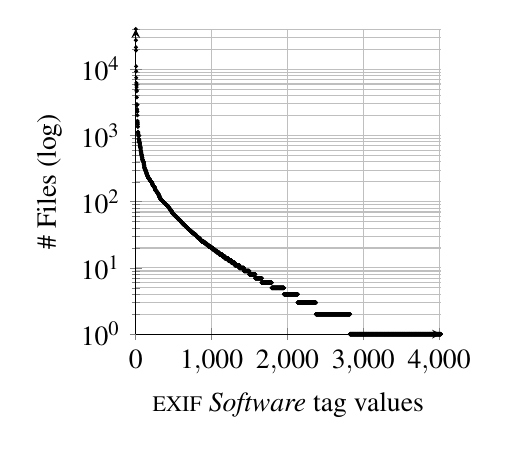
\begin{tikzpicture}
\begin{semilogyaxis}[ylabel={\# Files (log)},xlabel={\EXIF \textit{Software} tag values},grid=both, height=.45\columnwidth,width=0.45\columnwidth,xmin=0,axis x line=bottom, axis y line=left,cycle list name=black white]
\addplot [only marks, mark size=.5pt] coordinates {(1, 40480)
(2, 27423)
(3, 21417)
(4, 19226)
(5, 11052)
(6, 9312)
(7, 7443)
(8, 6242)
(9, 5986)
(10, 5759)
(11, 5370)
(12, 4819)
(13, 4673)
(14, 3768)
(15, 2965)
(16, 2852)
(17, 2508)
(18, 2442)
(19, 2299)
(20, 2284)
(21, 2019)
(22, 1665)
(23, 1647)
(24, 1546)
(25, 1545)
(26, 1461)
(27, 1372)
(28, 1347)
(29, 1137)
(30, 1127)
(31, 1126)
(32, 1096)
(33, 1061)
(34, 1022)
(35, 1021)
(36, 1013)
(37, 1004)
(38, 975)
(39, 897)
(40, 887)
(41, 876)
(42, 872)
(43, 866)
(44, 864)
(45, 846)
(46, 822)
(47, 795)
(48, 795)
(49, 793)
(50, 793)
(51, 787)
(52, 764)
(53, 755)
(54, 729)
(55, 697)
(56, 688)
(57, 685)
(58, 677)
(59, 676)
(60, 673)
(61, 660)
(62, 660)
(63, 646)
(64, 631)
(65, 606)
(66, 599)
(67, 586)
(68, 582)
(69, 578)
(70, 566)
(71, 558)
(72, 546)
(73, 528)
(74, 524)
(75, 521)
(76, 515)
(77, 509)
(78, 501)
(79, 496)
(80, 488)
(81, 483)
(82, 469)
(83, 467)
(84, 463)
(85, 462)
(86, 454)
(87, 439)
(88, 432)
(89, 432)
(90, 429)
(91, 427)
(92, 426)
(93, 423)
(94, 421)
(95, 420)
(96, 412)
(97, 408)
(98, 406)
(99, 405)
(100, 404)
(101, 401)
(102, 398)
(103, 397)
(104, 393)
(105, 387)
(106, 380)
(107, 367)
(108, 364)
(109, 362)
(110, 357)
(111, 352)
(112, 341)
(113, 333)
(114, 327)
(115, 327)
(116, 325)
(117, 322)
(118, 321)
(119, 316)
(120, 312)
(121, 312)
(122, 312)
(123, 312)
(124, 311)
(125, 308)
(126, 305)
(127, 299)
(128, 299)
(129, 298)
(130, 296)
(131, 293)
(132, 292)
(133, 289)
(134, 288)
(135, 287)
(136, 283)
(137, 280)
(138, 279)
(139, 277)
(140, 275)
(141, 272)
(142, 269)
(143, 268)
(144, 267)
(145, 263)
(146, 258)
(147, 258)
(148, 258)
(149, 258)
(150, 254)
(151, 252)
(152, 248)
(153, 247)
(154, 247)
(155, 246)
(156, 245)
(157, 244)
(158, 244)
(159, 242)
(160, 240)
(161, 239)
(162, 235)
(163, 235)
(164, 235)
(165, 230)
(166, 228)
(167, 228)
(168, 226)
(169, 226)
(170, 225)
(171, 225)
(172, 225)
(173, 224)
(174, 223)
(175, 223)
(176, 222)
(177, 222)
(178, 222)
(179, 221)
(180, 221)
(181, 220)
(182, 219)
(183, 218)
(184, 217)
(185, 214)
(186, 213)
(187, 211)
(188, 210)
(189, 210)
(190, 208)
(191, 208)
(192, 207)
(193, 207)
(194, 206)
(195, 205)
(196, 205)
(197, 204)
(198, 203)
(199, 203)
(200, 202)
(201, 202)
(202, 202)
(203, 201)
(204, 201)
(205, 201)
(206, 200)
(207, 200)
(208, 198)
(209, 198)
(210, 196)
(211, 195)
(212, 194)
(213, 194)
(214, 194)
(215, 194)
(216, 190)
(217, 189)
(218, 188)
(219, 186)
(220, 183)
(221, 182)
(222, 182)
(223, 181)
(224, 181)
(225, 177)
(226, 177)
(227, 176)
(228, 175)
(229, 175)
(230, 174)
(231, 174)
(232, 173)
(233, 173)
(234, 173)
(235, 172)
(236, 172)
(237, 171)
(238, 171)
(239, 171)
(240, 171)
(241, 170)
(242, 169)
(243, 169)
(244, 168)
(245, 167)
(246, 167)
(247, 167)
(248, 166)
(249, 163)
(250, 162)
(251, 161)
(252, 159)
(253, 158)
(254, 158)
(255, 157)
(256, 152)
(257, 151)
(258, 151)
(259, 151)
(260, 149)
(261, 149)
(262, 148)
(263, 148)
(264, 148)
(265, 146)
(266, 146)
(267, 145)
(268, 145)
(269, 144)
(270, 144)
(271, 144)
(272, 143)
(273, 143)
(274, 143)
(275, 143)
(276, 142)
(277, 142)
(278, 142)
(279, 142)
(280, 141)
(281, 141)
(282, 140)
(283, 138)
(284, 138)
(285, 137)
(286, 136)
(287, 136)
(288, 136)
(289, 136)
(290, 136)
(291, 134)
(292, 133)
(293, 133)
(294, 133)
(295, 132)
(296, 132)
(297, 131)
(298, 131)
(299, 130)
(300, 130)
(301, 128)
(302, 128)
(303, 127)
(304, 125)
(305, 125)
(306, 124)
(307, 123)
(308, 123)
(309, 122)
(310, 122)
(311, 121)
(312, 121)
(313, 118)
(314, 117)
(315, 116)
(316, 116)
(317, 115)
(318, 115)
(319, 115)
(320, 115)
(321, 115)
(322, 113)
(323, 112)
(324, 111)
(325, 111)
(326, 111)
(327, 110)
(328, 110)
(329, 108)
(330, 108)
(331, 108)
(332, 108)
(333, 107)
(334, 107)
(335, 107)
(336, 107)
(337, 106)
(338, 106)
(339, 106)
(340, 106)
(341, 106)
(342, 106)
(343, 106)
(344, 105)
(345, 105)
(346, 105)
(347, 105)
(348, 104)
(349, 104)
(350, 103)
(351, 103)
(352, 103)
(353, 103)
(354, 103)
(355, 102)
(356, 101)
(357, 101)
(358, 101)
(359, 101)
(360, 100)
(361, 100)
(362, 100)
(363, 100)
(364, 99)
(365, 99)
(366, 99)
(367, 99)
(368, 99)
(369, 99)
(370, 98)
(371, 98)
(372, 98)
(373, 97)
(374, 96)
(375, 96)
(376, 96)
(377, 95)
(378, 95)
(379, 95)
(380, 95)
(381, 94)
(382, 94)
(383, 94)
(384, 94)
(385, 94)
(386, 94)
(387, 94)
(388, 93)
(389, 93)
(390, 93)
(391, 93)
(392, 92)
(393, 92)
(394, 91)
(395, 91)
(396, 91)
(397, 91)
(398, 90)
(399, 90)
(400, 90)
(401, 90)
(402, 90)
(403, 90)
(404, 89)
(405, 89)
(406, 89)
(407, 89)
(408, 89)
(409, 89)
(410, 89)
(411, 88)
(412, 88)
(413, 88)
(414, 88)
(415, 88)
(416, 88)
(417, 88)
(418, 88)
(419, 88)
(420, 86)
(421, 86)
(422, 86)
(423, 86)
(424, 85)
(425, 85)
(426, 85)
(427, 85)
(428, 85)
(429, 85)
(430, 83)
(431, 83)
(432, 83)
(433, 83)
(434, 82)
(435, 82)
(436, 81)
(437, 81)
(438, 81)
(439, 81)
(440, 80)
(441, 80)
(442, 80)
(443, 80)
(444, 79)
(445, 79)
(446, 79)
(447, 79)
(448, 78)
(449, 78)
(450, 78)
(451, 77)
(452, 77)
(453, 77)
(454, 77)
(455, 76)
(456, 76)
(457, 76)
(458, 76)
(459, 75)
(460, 75)
(461, 75)
(462, 75)
(463, 75)
(464, 75)
(465, 74)
(466, 73)
(467, 73)
(468, 73)
(469, 73)
(470, 73)
(471, 72)
(472, 72)
(473, 72)
(474, 72)
(475, 70)
(476, 70)
(477, 70)
(478, 69)
(479, 69)
(480, 68)
(481, 68)
(482, 68)
(483, 67)
(484, 67)
(485, 67)
(486, 67)
(487, 67)
(488, 66)
(489, 66)
(490, 66)
(491, 66)
(492, 66)
(493, 66)
(494, 65)
(495, 65)
(496, 65)
(497, 65)
(498, 65)
(499, 65)
(500, 65)
(501, 64)
(502, 64)
(503, 64)
(504, 64)
(505, 63)
(506, 63)
(507, 63)
(508, 63)
(509, 63)
(510, 63)
(511, 63)
(512, 63)
(513, 62)
(514, 62)
(515, 62)
(516, 61)
(517, 61)
(518, 61)
(519, 61)
(520, 61)
(521, 61)
(522, 61)
(523, 60)
(524, 60)
(525, 60)
(526, 60)
(527, 60)
(528, 60)
(529, 60)
(530, 60)
(531, 60)
(532, 60)
(533, 60)
(534, 60)
(535, 60)
(536, 60)
(537, 59)
(538, 59)
(539, 59)
(540, 59)
(541, 59)
(542, 58)
(543, 58)
(544, 58)
(545, 57)
(546, 57)
(547, 57)
(548, 57)
(549, 57)
(550, 57)
(551, 57)
(552, 57)
(553, 56)
(554, 56)
(555, 56)
(556, 56)
(557, 55)
(558, 55)
(559, 55)
(560, 55)
(561, 55)
(562, 54)
(563, 54)
(564, 54)
(565, 54)
(566, 54)
(567, 54)
(568, 54)
(569, 54)
(570, 54)
(571, 54)
(572, 54)
(573, 54)
(574, 53)
(575, 53)
(576, 53)
(577, 53)
(578, 53)
(579, 53)
(580, 53)
(581, 53)
(582, 53)
(583, 53)
(584, 52)
(585, 52)
(586, 52)
(587, 52)
(588, 52)
(589, 52)
(590, 52)
(591, 52)
(592, 51)
(593, 51)
(594, 51)
(595, 50)
(596, 50)
(597, 50)
(598, 50)
(599, 50)
(600, 49)
(601, 49)
(602, 49)
(603, 49)
(604, 49)
(605, 49)
(606, 49)
(607, 48)
(608, 48)
(609, 48)
(610, 48)
(611, 48)
(612, 48)
(613, 48)
(614, 48)
(615, 48)
(616, 47)
(617, 47)
(618, 47)
(619, 47)
(620, 47)
(621, 47)
(622, 46)
(623, 46)
(624, 46)
(625, 46)
(626, 46)
(627, 46)
(628, 46)
(629, 45)
(630, 45)
(631, 45)
(632, 45)
(633, 45)
(634, 45)
(635, 45)
(636, 45)
(637, 45)
(638, 45)
(639, 45)
(640, 45)
(641, 44)
(642, 44)
(643, 44)
(644, 44)
(645, 44)
(646, 44)
(647, 44)
(648, 44)
(649, 44)
(650, 44)
(651, 43)
(652, 43)
(653, 43)
(654, 43)
(655, 43)
(656, 43)
(657, 43)
(658, 43)
(659, 43)
(660, 42)
(661, 42)
(662, 42)
(663, 42)
(664, 42)
(665, 42)
(666, 42)
(667, 42)
(668, 42)
(669, 42)
(670, 41)
(671, 41)
(672, 41)
(673, 41)
(674, 41)
(675, 41)
(676, 41)
(677, 40)
(678, 40)
(679, 40)
(680, 40)
(681, 40)
(682, 40)
(683, 40)
(684, 40)
(685, 40)
(686, 39)
(687, 39)
(688, 39)
(689, 39)
(690, 39)
(691, 39)
(692, 39)
(693, 39)
(694, 39)
(695, 39)
(696, 39)
(697, 38)
(698, 38)
(699, 38)
(700, 38)
(701, 38)
(702, 38)
(703, 38)
(704, 38)
(705, 38)
(706, 38)
(707, 38)
(708, 38)
(709, 37)
(710, 37)
(711, 37)
(712, 37)
(713, 37)
(714, 37)
(715, 37)
(716, 37)
(717, 37)
(718, 37)
(719, 37)
(720, 36)
(721, 36)
(722, 36)
(723, 36)
(724, 36)
(725, 36)
(726, 36)
(727, 36)
(728, 36)
(729, 36)
(730, 36)
(731, 36)
(732, 36)
(733, 36)
(734, 35)
(735, 35)
(736, 35)
(737, 35)
(738, 35)
(739, 35)
(740, 35)
(741, 35)
(742, 35)
(743, 34)
(744, 34)
(745, 34)
(746, 34)
(747, 34)
(748, 34)
(749, 34)
(750, 34)
(751, 34)
(752, 34)
(753, 34)
(754, 34)
(755, 34)
(756, 34)
(757, 33)
(758, 33)
(759, 33)
(760, 33)
(761, 33)
(762, 33)
(763, 33)
(764, 33)
(765, 33)
(766, 33)
(767, 33)
(768, 33)
(769, 33)
(770, 33)
(771, 33)
(772, 32)
(773, 32)
(774, 32)
(775, 32)
(776, 32)
(777, 32)
(778, 32)
(779, 32)
(780, 32)
(781, 32)
(782, 32)
(783, 32)
(784, 32)
(785, 32)
(786, 32)
(787, 32)
(788, 32)
(789, 32)
(790, 32)
(791, 31)
(792, 31)
(793, 31)
(794, 31)
(795, 31)
(796, 31)
(797, 31)
(798, 31)
(799, 31)
(800, 31)
(801, 30)
(802, 30)
(803, 30)
(804, 30)
(805, 30)
(806, 30)
(807, 30)
(808, 30)
(809, 30)
(810, 29)
(811, 29)
(812, 29)
(813, 29)
(814, 29)
(815, 29)
(816, 29)
(817, 29)
(818, 29)
(819, 29)
(820, 29)
(821, 29)
(822, 29)
(823, 29)
(824, 29)
(825, 29)
(826, 29)
(827, 29)
(828, 29)
(829, 29)
(830, 28)
(831, 28)
(832, 28)
(833, 28)
(834, 28)
(835, 28)
(836, 28)
(837, 28)
(838, 28)
(839, 28)
(840, 28)
(841, 28)
(842, 28)
(843, 28)
(844, 28)
(845, 28)
(846, 27)
(847, 27)
(848, 27)
(849, 27)
(850, 27)
(851, 27)
(852, 27)
(853, 27)
(854, 27)
(855, 27)
(856, 26)
(857, 26)
(858, 26)
(859, 26)
(860, 26)
(861, 26)
(862, 26)
(863, 26)
(864, 26)
(865, 26)
(866, 26)
(867, 26)
(868, 26)
(869, 26)
(870, 25)
(871, 25)
(872, 25)
(873, 25)
(874, 25)
(875, 25)
(876, 25)
(877, 25)
(878, 25)
(879, 25)
(880, 25)
(881, 25)
(882, 25)
(883, 25)
(884, 25)
(885, 25)
(886, 25)
(887, 25)
(888, 25)
(889, 25)
(890, 25)
(891, 25)
(892, 25)
(893, 25)
(894, 25)
(895, 25)
(896, 25)
(897, 25)
(898, 24)
(899, 24)
(900, 24)
(901, 24)
(902, 24)
(903, 24)
(904, 24)
(905, 24)
(906, 24)
(907, 24)
(908, 24)
(909, 24)
(910, 24)
(911, 24)
(912, 24)
(913, 24)
(914, 24)
(915, 24)
(916, 24)
(917, 24)
(918, 24)
(919, 23)
(920, 23)
(921, 23)
(922, 23)
(923, 23)
(924, 23)
(925, 23)
(926, 23)
(927, 23)
(928, 23)
(929, 23)
(930, 23)
(931, 23)
(932, 23)
(933, 23)
(934, 23)
(935, 23)
(936, 23)
(937, 23)
(938, 23)
(939, 23)
(940, 23)
(941, 23)
(942, 23)
(943, 22)
(944, 22)
(945, 22)
(946, 22)
(947, 22)
(948, 22)
(949, 22)
(950, 22)
(951, 22)
(952, 22)
(953, 22)
(954, 22)
(955, 22)
(956, 22)
(957, 22)
(958, 22)
(959, 22)
(960, 22)
(961, 22)
(962, 22)
(963, 21)
(964, 21)
(965, 21)
(966, 21)
(967, 21)
(968, 21)
(969, 21)
(970, 21)
(971, 21)
(972, 21)
(973, 21)
(974, 21)
(975, 21)
(976, 21)
(977, 21)
(978, 21)
(979, 21)
(980, 21)
(981, 21)
(982, 21)
(983, 21)
(984, 21)
(985, 21)
(986, 21)
(987, 21)
(988, 21)
(989, 21)
(990, 21)
(991, 20)
(992, 20)
(993, 20)
(994, 20)
(995, 20)
(996, 20)
(997, 20)
(998, 20)
(999, 20)
(1000, 20)
(1001, 20)
(1002, 20)
(1003, 20)
(1004, 20)
(1005, 20)
(1006, 20)
(1007, 20)
(1008, 20)
(1009, 20)
(1010, 20)
(1011, 20)
(1012, 20)
(1013, 20)
(1014, 20)
(1015, 20)
(1016, 20)
(1017, 20)
(1018, 19)
(1019, 19)
(1020, 19)
(1021, 19)
(1022, 19)
(1023, 19)
(1024, 19)
(1025, 19)
(1026, 19)
(1027, 19)
(1028, 19)
(1029, 19)
(1030, 19)
(1031, 19)
(1032, 19)
(1033, 19)
(1034, 19)
(1035, 19)
(1036, 19)
(1037, 19)
(1038, 19)
(1039, 19)
(1040, 19)
(1041, 19)
(1042, 19)
(1043, 18)
(1044, 18)
(1045, 18)
(1046, 18)
(1047, 18)
(1048, 18)
(1049, 18)
(1050, 18)
(1051, 18)
(1052, 18)
(1053, 18)
(1054, 18)
(1055, 18)
(1056, 18)
(1057, 18)
(1058, 18)
(1059, 18)
(1060, 18)
(1061, 18)
(1062, 18)
(1063, 18)
(1064, 18)
(1065, 18)
(1066, 18)
(1067, 18)
(1068, 18)
(1069, 18)
(1070, 18)
(1071, 18)
(1072, 18)
(1073, 17)
(1074, 17)
(1075, 17)
(1076, 17)
(1077, 17)
(1078, 17)
(1079, 17)
(1080, 17)
(1081, 17)
(1082, 17)
(1083, 17)
(1084, 17)
(1085, 17)
(1086, 17)
(1087, 17)
(1088, 17)
(1089, 17)
(1090, 17)
(1091, 17)
(1092, 17)
(1093, 17)
(1094, 17)
(1095, 17)
(1096, 17)
(1097, 17)
(1098, 17)
(1099, 17)
(1100, 17)
(1101, 17)
(1102, 16)
(1103, 16)
(1104, 16)
(1105, 16)
(1106, 16)
(1107, 16)
(1108, 16)
(1109, 16)
(1110, 16)
(1111, 16)
(1112, 16)
(1113, 16)
(1114, 16)
(1115, 16)
(1116, 16)
(1117, 16)
(1118, 16)
(1119, 16)
(1120, 16)
(1121, 16)
(1122, 16)
(1123, 16)
(1124, 16)
(1125, 16)
(1126, 16)
(1127, 16)
(1128, 16)
(1129, 16)
(1130, 16)
(1131, 16)
(1132, 16)
(1133, 16)
(1134, 16)
(1135, 16)
(1136, 16)
(1137, 16)
(1138, 16)
(1139, 16)
(1140, 15)
(1141, 15)
(1142, 15)
(1143, 15)
(1144, 15)
(1145, 15)
(1146, 15)
(1147, 15)
(1148, 15)
(1149, 15)
(1150, 15)
(1151, 15)
(1152, 15)
(1153, 15)
(1154, 15)
(1155, 15)
(1156, 15)
(1157, 15)
(1158, 15)
(1159, 15)
(1160, 15)
(1161, 15)
(1162, 15)
(1163, 15)
(1164, 15)
(1165, 15)
(1166, 15)
(1167, 15)
(1168, 15)
(1169, 15)
(1170, 15)
(1171, 15)
(1172, 15)
(1173, 15)
(1174, 14)
(1175, 14)
(1176, 14)
(1177, 14)
(1178, 14)
(1179, 14)
(1180, 14)
(1181, 14)
(1182, 14)
(1183, 14)
(1184, 14)
(1185, 14)
(1186, 14)
(1187, 14)
(1188, 14)
(1189, 14)
(1190, 14)
(1191, 14)
(1192, 14)
(1193, 14)
(1194, 14)
(1195, 14)
(1196, 14)
(1197, 14)
(1198, 14)
(1199, 14)
(1200, 14)
(1201, 14)
(1202, 14)
(1203, 14)
(1204, 14)
(1205, 14)
(1206, 14)
(1207, 14)
(1208, 14)
(1209, 14)
(1210, 14)
(1211, 14)
(1212, 14)
(1213, 14)
(1214, 14)
(1215, 14)
(1216, 14)
(1217, 14)
(1218, 13)
(1219, 13)
(1220, 13)
(1221, 13)
(1222, 13)
(1223, 13)
(1224, 13)
(1225, 13)
(1226, 13)
(1227, 13)
(1228, 13)
(1229, 13)
(1230, 13)
(1231, 13)
(1232, 13)
(1233, 13)
(1234, 13)
(1235, 13)
(1236, 13)
(1237, 13)
(1238, 13)
(1239, 13)
(1240, 13)
(1241, 13)
(1242, 13)
(1243, 13)
(1244, 13)
(1245, 13)
(1246, 13)
(1247, 13)
(1248, 13)
(1249, 13)
(1250, 13)
(1251, 13)
(1252, 13)
(1253, 13)
(1254, 13)
(1255, 13)
(1256, 13)
(1257, 13)
(1258, 13)
(1259, 13)
(1260, 13)
(1261, 13)
(1262, 12)
(1263, 12)
(1264, 12)
(1265, 12)
(1266, 12)
(1267, 12)
(1268, 12)
(1269, 12)
(1270, 12)
(1271, 12)
(1272, 12)
(1273, 12)
(1274, 12)
(1275, 12)
(1276, 12)
(1277, 12)
(1278, 12)
(1279, 12)
(1280, 12)
(1281, 12)
(1282, 12)
(1283, 12)
(1284, 12)
(1285, 12)
(1286, 12)
(1287, 12)
(1288, 12)
(1289, 12)
(1290, 12)
(1291, 12)
(1292, 12)
(1293, 12)
(1294, 12)
(1295, 12)
(1296, 12)
(1297, 12)
(1298, 12)
(1299, 12)
(1300, 12)
(1301, 12)
(1302, 12)
(1303, 12)
(1304, 12)
(1305, 12)
(1306, 11)
(1307, 11)
(1308, 11)
(1309, 11)
(1310, 11)
(1311, 11)
(1312, 11)
(1313, 11)
(1314, 11)
(1315, 11)
(1316, 11)
(1317, 11)
(1318, 11)
(1319, 11)
(1320, 11)
(1321, 11)
(1322, 11)
(1323, 11)
(1324, 11)
(1325, 11)
(1326, 11)
(1327, 11)
(1328, 11)
(1329, 11)
(1330, 11)
(1331, 11)
(1332, 11)
(1333, 11)
(1334, 11)
(1335, 11)
(1336, 11)
(1337, 11)
(1338, 11)
(1339, 11)
(1340, 11)
(1341, 11)
(1342, 11)
(1343, 11)
(1344, 11)
(1345, 11)
(1346, 11)
(1347, 11)
(1348, 11)
(1349, 11)
(1350, 11)
(1351, 11)
(1352, 11)
(1353, 11)
(1354, 11)
(1355, 11)
(1356, 11)
(1357, 11)
(1358, 11)
(1359, 11)
(1360, 11)
(1361, 11)
(1362, 11)
(1363, 11)
(1364, 11)
(1365, 11)
(1366, 10)
(1367, 10)
(1368, 10)
(1369, 10)
(1370, 10)
(1371, 10)
(1372, 10)
(1373, 10)
(1374, 10)
(1375, 10)
(1376, 10)
(1377, 10)
(1378, 10)
(1379, 10)
(1380, 10)
(1381, 10)
(1382, 10)
(1383, 10)
(1384, 10)
(1385, 10)
(1386, 10)
(1387, 10)
(1388, 10)
(1389, 10)
(1390, 10)
(1391, 10)
(1392, 10)
(1393, 10)
(1394, 10)
(1395, 10)
(1396, 10)
(1397, 10)
(1398, 10)
(1399, 10)
(1400, 10)
(1401, 10)
(1402, 10)
(1403, 10)
(1404, 10)
(1405, 10)
(1406, 10)
(1407, 10)
(1408, 10)
(1409, 10)
(1410, 10)
(1411, 10)
(1412, 10)
(1413, 10)
(1414, 10)
(1415, 10)
(1416, 10)
(1417, 10)
(1418, 10)
(1419, 10)
(1420, 10)
(1421, 10)
(1422, 10)
(1423, 10)
(1424, 10)
(1425, 10)
(1426, 9)
(1427, 9)
(1428, 9)
(1429, 9)
(1430, 9)
(1431, 9)
(1432, 9)
(1433, 9)
(1434, 9)
(1435, 9)
(1436, 9)
(1437, 9)
(1438, 9)
(1439, 9)
(1440, 9)
(1441, 9)
(1442, 9)
(1443, 9)
(1444, 9)
(1445, 9)
(1446, 9)
(1447, 9)
(1448, 9)
(1449, 9)
(1450, 9)
(1451, 9)
(1452, 9)
(1453, 9)
(1454, 9)
(1455, 9)
(1456, 9)
(1457, 9)
(1458, 9)
(1459, 9)
(1460, 9)
(1461, 9)
(1462, 9)
(1463, 9)
(1464, 9)
(1465, 9)
(1466, 9)
(1467, 9)
(1468, 9)
(1469, 9)
(1470, 9)
(1471, 9)
(1472, 9)
(1473, 9)
(1474, 9)
(1475, 9)
(1476, 9)
(1477, 9)
(1478, 9)
(1479, 9)
(1480, 9)
(1481, 9)
(1482, 9)
(1483, 9)
(1484, 9)
(1485, 9)
(1486, 9)
(1487, 9)
(1488, 9)
(1489, 9)
(1490, 9)
(1491, 9)
(1492, 9)
(1493, 9)
(1494, 9)
(1495, 9)
(1496, 9)
(1497, 8)
(1498, 8)
(1499, 8)
(1500, 8)
(1501, 8)
(1502, 8)
(1503, 8)
(1504, 8)
(1505, 8)
(1506, 8)
(1507, 8)
(1508, 8)
(1509, 8)
(1510, 8)
(1511, 8)
(1512, 8)
(1513, 8)
(1514, 8)
(1515, 8)
(1516, 8)
(1517, 8)
(1518, 8)
(1519, 8)
(1520, 8)
(1521, 8)
(1522, 8)
(1523, 8)
(1524, 8)
(1525, 8)
(1526, 8)
(1527, 8)
(1528, 8)
(1529, 8)
(1530, 8)
(1531, 8)
(1532, 8)
(1533, 8)
(1534, 8)
(1535, 8)
(1536, 8)
(1537, 8)
(1538, 8)
(1539, 8)
(1540, 8)
(1541, 8)
(1542, 8)
(1543, 8)
(1544, 8)
(1545, 8)
(1546, 8)
(1547, 8)
(1548, 8)
(1549, 8)
(1550, 8)
(1551, 8)
(1552, 8)
(1553, 8)
(1554, 8)
(1555, 8)
(1556, 8)
(1557, 8)
(1558, 8)
(1559, 8)
(1560, 8)
(1561, 8)
(1562, 8)
(1563, 8)
(1564, 8)
(1565, 8)
(1566, 8)
(1567, 8)
(1568, 8)
(1569, 8)
(1570, 8)
(1571, 8)
(1572, 8)
(1573, 8)
(1574, 8)
(1575, 8)
(1576, 7)
(1577, 7)
(1578, 7)
(1579, 7)
(1580, 7)
(1581, 7)
(1582, 7)
(1583, 7)
(1584, 7)
(1585, 7)
(1586, 7)
(1587, 7)
(1588, 7)
(1589, 7)
(1590, 7)
(1591, 7)
(1592, 7)
(1593, 7)
(1594, 7)
(1595, 7)
(1596, 7)
(1597, 7)
(1598, 7)
(1599, 7)
(1600, 7)
(1601, 7)
(1602, 7)
(1603, 7)
(1604, 7)
(1605, 7)
(1606, 7)
(1607, 7)
(1608, 7)
(1609, 7)
(1610, 7)
(1611, 7)
(1612, 7)
(1613, 7)
(1614, 7)
(1615, 7)
(1616, 7)
(1617, 7)
(1618, 7)
(1619, 7)
(1620, 7)
(1621, 7)
(1622, 7)
(1623, 7)
(1624, 7)
(1625, 7)
(1626, 7)
(1627, 7)
(1628, 7)
(1629, 7)
(1630, 7)
(1631, 7)
(1632, 7)
(1633, 7)
(1634, 7)
(1635, 7)
(1636, 7)
(1637, 7)
(1638, 7)
(1639, 7)
(1640, 7)
(1641, 7)
(1642, 7)
(1643, 7)
(1644, 7)
(1645, 7)
(1646, 7)
(1647, 7)
(1648, 7)
(1649, 7)
(1650, 7)
(1651, 7)
(1652, 7)
(1653, 7)
(1654, 7)
(1655, 7)
(1656, 7)
(1657, 7)
(1658, 7)
(1659, 7)
(1660, 7)
(1661, 6)
(1662, 6)
(1663, 6)
(1664, 6)
(1665, 6)
(1666, 6)
(1667, 6)
(1668, 6)
(1669, 6)
(1670, 6)
(1671, 6)
(1672, 6)
(1673, 6)
(1674, 6)
(1675, 6)
(1676, 6)
(1677, 6)
(1678, 6)
(1679, 6)
(1680, 6)
(1681, 6)
(1682, 6)
(1683, 6)
(1684, 6)
(1685, 6)
(1686, 6)
(1687, 6)
(1688, 6)
(1689, 6)
(1690, 6)
(1691, 6)
(1692, 6)
(1693, 6)
(1694, 6)
(1695, 6)
(1696, 6)
(1697, 6)
(1698, 6)
(1699, 6)
(1700, 6)
(1701, 6)
(1702, 6)
(1703, 6)
(1704, 6)
(1705, 6)
(1706, 6)
(1707, 6)
(1708, 6)
(1709, 6)
(1710, 6)
(1711, 6)
(1712, 6)
(1713, 6)
(1714, 6)
(1715, 6)
(1716, 6)
(1717, 6)
(1718, 6)
(1719, 6)
(1720, 6)
(1721, 6)
(1722, 6)
(1723, 6)
(1724, 6)
(1725, 6)
(1726, 6)
(1727, 6)
(1728, 6)
(1729, 6)
(1730, 6)
(1731, 6)
(1732, 6)
(1733, 6)
(1734, 6)
(1735, 6)
(1736, 6)
(1737, 6)
(1738, 6)
(1739, 6)
(1740, 6)
(1741, 6)
(1742, 6)
(1743, 6)
(1744, 6)
(1745, 6)
(1746, 6)
(1747, 6)
(1748, 6)
(1749, 6)
(1750, 6)
(1751, 6)
(1752, 6)
(1753, 6)
(1754, 6)
(1755, 6)
(1756, 6)
(1757, 6)
(1758, 6)
(1759, 6)
(1760, 6)
(1761, 6)
(1762, 6)
(1763, 6)
(1764, 6)
(1765, 6)
(1766, 6)
(1767, 6)
(1768, 6)
(1769, 6)
(1770, 6)
(1771, 6)
(1772, 6)
(1773, 6)
(1774, 6)
(1775, 6)
(1776, 6)
(1777, 6)
(1778, 6)
(1779, 6)
(1780, 6)
(1781, 6)
(1782, 6)
(1783, 6)
(1784, 6)
(1785, 6)
(1786, 6)
(1787, 6)
(1788, 6)
(1789, 6)
(1790, 6)
(1791, 6)
(1792, 6)
(1793, 5)
(1794, 5)
(1795, 5)
(1796, 5)
(1797, 5)
(1798, 5)
(1799, 5)
(1800, 5)
(1801, 5)
(1802, 5)
(1803, 5)
(1804, 5)
(1805, 5)
(1806, 5)
(1807, 5)
(1808, 5)
(1809, 5)
(1810, 5)
(1811, 5)
(1812, 5)
(1813, 5)
(1814, 5)
(1815, 5)
(1816, 5)
(1817, 5)
(1818, 5)
(1819, 5)
(1820, 5)
(1821, 5)
(1822, 5)
(1823, 5)
(1824, 5)
(1825, 5)
(1826, 5)
(1827, 5)
(1828, 5)
(1829, 5)
(1830, 5)
(1831, 5)
(1832, 5)
(1833, 5)
(1834, 5)
(1835, 5)
(1836, 5)
(1837, 5)
(1838, 5)
(1839, 5)
(1840, 5)
(1841, 5)
(1842, 5)
(1843, 5)
(1844, 5)
(1845, 5)
(1846, 5)
(1847, 5)
(1848, 5)
(1849, 5)
(1850, 5)
(1851, 5)
(1852, 5)
(1853, 5)
(1854, 5)
(1855, 5)
(1856, 5)
(1857, 5)
(1858, 5)
(1859, 5)
(1860, 5)
(1861, 5)
(1862, 5)
(1863, 5)
(1864, 5)
(1865, 5)
(1866, 5)
(1867, 5)
(1868, 5)
(1869, 5)
(1870, 5)
(1871, 5)
(1872, 5)
(1873, 5)
(1874, 5)
(1875, 5)
(1876, 5)
(1877, 5)
(1878, 5)
(1879, 5)
(1880, 5)
(1881, 5)
(1882, 5)
(1883, 5)
(1884, 5)
(1885, 5)
(1886, 5)
(1887, 5)
(1888, 5)
(1889, 5)
(1890, 5)
(1891, 5)
(1892, 5)
(1893, 5)
(1894, 5)
(1895, 5)
(1896, 5)
(1897, 5)
(1898, 5)
(1899, 5)
(1900, 5)
(1901, 5)
(1902, 5)
(1903, 5)
(1904, 5)
(1905, 5)
(1906, 5)
(1907, 5)
(1908, 5)
(1909, 5)
(1910, 5)
(1911, 5)
(1912, 5)
(1913, 5)
(1914, 5)
(1915, 5)
(1916, 5)
(1917, 5)
(1918, 5)
(1919, 5)
(1920, 5)
(1921, 5)
(1922, 5)
(1923, 5)
(1924, 5)
(1925, 5)
(1926, 5)
(1927, 5)
(1928, 5)
(1929, 5)
(1930, 5)
(1931, 5)
(1932, 5)
(1933, 5)
(1934, 5)
(1935, 5)
(1936, 5)
(1937, 5)
(1938, 5)
(1939, 5)
(1940, 5)
(1941, 5)
(1942, 5)
(1943, 5)
(1944, 5)
(1945, 5)
(1946, 5)
(1947, 5)
(1948, 5)
(1949, 5)
(1950, 5)
(1951, 5)
(1952, 5)
(1953, 5)
(1954, 5)
(1955, 4)
(1956, 4)
(1957, 4)
(1958, 4)
(1959, 4)
(1960, 4)
(1961, 4)
(1962, 4)
(1963, 4)
(1964, 4)
(1965, 4)
(1966, 4)
(1967, 4)
(1968, 4)
(1969, 4)
(1970, 4)
(1971, 4)
(1972, 4)
(1973, 4)
(1974, 4)
(1975, 4)
(1976, 4)
(1977, 4)
(1978, 4)
(1979, 4)
(1980, 4)
(1981, 4)
(1982, 4)
(1983, 4)
(1984, 4)
(1985, 4)
(1986, 4)
(1987, 4)
(1988, 4)
(1989, 4)
(1990, 4)
(1991, 4)
(1992, 4)
(1993, 4)
(1994, 4)
(1995, 4)
(1996, 4)
(1997, 4)
(1998, 4)
(1999, 4)
(2000, 4)
(2001, 4)
(2002, 4)
(2003, 4)
(2004, 4)
(2005, 4)
(2006, 4)
(2007, 4)
(2008, 4)
(2009, 4)
(2010, 4)
(2011, 4)
(2012, 4)
(2013, 4)
(2014, 4)
(2015, 4)
(2016, 4)
(2017, 4)
(2018, 4)
(2019, 4)
(2020, 4)
(2021, 4)
(2022, 4)
(2023, 4)
(2024, 4)
(2025, 4)
(2026, 4)
(2027, 4)
(2028, 4)
(2029, 4)
(2030, 4)
(2031, 4)
(2032, 4)
(2033, 4)
(2034, 4)
(2035, 4)
(2036, 4)
(2037, 4)
(2038, 4)
(2039, 4)
(2040, 4)
(2041, 4)
(2042, 4)
(2043, 4)
(2044, 4)
(2045, 4)
(2046, 4)
(2047, 4)
(2048, 4)
(2049, 4)
(2050, 4)
(2051, 4)
(2052, 4)
(2053, 4)
(2054, 4)
(2055, 4)
(2056, 4)
(2057, 4)
(2058, 4)
(2059, 4)
(2060, 4)
(2061, 4)
(2062, 4)
(2063, 4)
(2064, 4)
(2065, 4)
(2066, 4)
(2067, 4)
(2068, 4)
(2069, 4)
(2070, 4)
(2071, 4)
(2072, 4)
(2073, 4)
(2074, 4)
(2075, 4)
(2076, 4)
(2077, 4)
(2078, 4)
(2079, 4)
(2080, 4)
(2081, 4)
(2082, 4)
(2083, 4)
(2084, 4)
(2085, 4)
(2086, 4)
(2087, 4)
(2088, 4)
(2089, 4)
(2090, 4)
(2091, 4)
(2092, 4)
(2093, 4)
(2094, 4)
(2095, 4)
(2096, 4)
(2097, 4)
(2098, 4)
(2099, 4)
(2100, 4)
(2101, 4)
(2102, 4)
(2103, 4)
(2104, 4)
(2105, 4)
(2106, 4)
(2107, 4)
(2108, 4)
(2109, 4)
(2110, 4)
(2111, 4)
(2112, 4)
(2113, 4)
(2114, 4)
(2115, 4)
(2116, 4)
(2117, 4)
(2118, 4)
(2119, 4)
(2120, 4)
(2121, 4)
(2122, 4)
(2123, 4)
(2124, 4)
(2125, 4)
(2126, 4)
(2127, 4)
(2128, 4)
(2129, 4)
(2130, 4)
(2131, 4)
(2132, 4)
(2133, 4)
(2134, 4)
(2135, 4)
(2136, 3)
(2137, 3)
(2138, 3)
(2139, 3)
(2140, 3)
(2141, 3)
(2142, 3)
(2143, 3)
(2144, 3)
(2145, 3)
(2146, 3)
(2147, 3)
(2148, 3)
(2149, 3)
(2150, 3)
(2151, 3)
(2152, 3)
(2153, 3)
(2154, 3)
(2155, 3)
(2156, 3)
(2157, 3)
(2158, 3)
(2159, 3)
(2160, 3)
(2161, 3)
(2162, 3)
(2163, 3)
(2164, 3)
(2165, 3)
(2166, 3)
(2167, 3)
(2168, 3)
(2169, 3)
(2170, 3)
(2171, 3)
(2172, 3)
(2173, 3)
(2174, 3)
(2175, 3)
(2176, 3)
(2177, 3)
(2178, 3)
(2179, 3)
(2180, 3)
(2181, 3)
(2182, 3)
(2183, 3)
(2184, 3)
(2185, 3)
(2186, 3)
(2187, 3)
(2188, 3)
(2189, 3)
(2190, 3)
(2191, 3)
(2192, 3)
(2193, 3)
(2194, 3)
(2195, 3)
(2196, 3)
(2197, 3)
(2198, 3)
(2199, 3)
(2200, 3)
(2201, 3)
(2202, 3)
(2203, 3)
(2204, 3)
(2205, 3)
(2206, 3)
(2207, 3)
(2208, 3)
(2209, 3)
(2210, 3)
(2211, 3)
(2212, 3)
(2213, 3)
(2214, 3)
(2215, 3)
(2216, 3)
(2217, 3)
(2218, 3)
(2219, 3)
(2220, 3)
(2221, 3)
(2222, 3)
(2223, 3)
(2224, 3)
(2225, 3)
(2226, 3)
(2227, 3)
(2228, 3)
(2229, 3)
(2230, 3)
(2231, 3)
(2232, 3)
(2233, 3)
(2234, 3)
(2235, 3)
(2236, 3)
(2237, 3)
(2238, 3)
(2239, 3)
(2240, 3)
(2241, 3)
(2242, 3)
(2243, 3)
(2244, 3)
(2245, 3)
(2246, 3)
(2247, 3)
(2248, 3)
(2249, 3)
(2250, 3)
(2251, 3)
(2252, 3)
(2253, 3)
(2254, 3)
(2255, 3)
(2256, 3)
(2257, 3)
(2258, 3)
(2259, 3)
(2260, 3)
(2261, 3)
(2262, 3)
(2263, 3)
(2264, 3)
(2265, 3)
(2266, 3)
(2267, 3)
(2268, 3)
(2269, 3)
(2270, 3)
(2271, 3)
(2272, 3)
(2273, 3)
(2274, 3)
(2275, 3)
(2276, 3)
(2277, 3)
(2278, 3)
(2279, 3)
(2280, 3)
(2281, 3)
(2282, 3)
(2283, 3)
(2284, 3)
(2285, 3)
(2286, 3)
(2287, 3)
(2288, 3)
(2289, 3)
(2290, 3)
(2291, 3)
(2292, 3)
(2293, 3)
(2294, 3)
(2295, 3)
(2296, 3)
(2297, 3)
(2298, 3)
(2299, 3)
(2300, 3)
(2301, 3)
(2302, 3)
(2303, 3)
(2304, 3)
(2305, 3)
(2306, 3)
(2307, 3)
(2308, 3)
(2309, 3)
(2310, 3)
(2311, 3)
(2312, 3)
(2313, 3)
(2314, 3)
(2315, 3)
(2316, 3)
(2317, 3)
(2318, 3)
(2319, 3)
(2320, 3)
(2321, 3)
(2322, 3)
(2323, 3)
(2324, 3)
(2325, 3)
(2326, 3)
(2327, 3)
(2328, 3)
(2329, 3)
(2330, 3)
(2331, 3)
(2332, 3)
(2333, 3)
(2334, 3)
(2335, 3)
(2336, 3)
(2337, 3)
(2338, 3)
(2339, 3)
(2340, 3)
(2341, 3)
(2342, 3)
(2343, 3)
(2344, 3)
(2345, 3)
(2346, 3)
(2347, 3)
(2348, 3)
(2349, 3)
(2350, 3)
(2351, 3)
(2352, 3)
(2353, 3)
(2354, 3)
(2355, 3)
(2356, 3)
(2357, 3)
(2358, 3)
(2359, 3)
(2360, 3)
(2361, 3)
(2362, 3)
(2363, 3)
(2364, 3)
(2365, 3)
(2366, 3)
(2367, 3)
(2368, 3)
(2369, 3)
(2370, 3)
(2371, 3)
(2372, 3)
(2373, 3)
(2374, 3)
(2375, 3)
(2376, 2)
(2377, 2)
(2378, 2)
(2379, 2)
(2380, 2)
(2381, 2)
(2382, 2)
(2383, 2)
(2384, 2)
(2385, 2)
(2386, 2)
(2387, 2)
(2388, 2)
(2389, 2)
(2390, 2)
(2391, 2)
(2392, 2)
(2393, 2)
(2394, 2)
(2395, 2)
(2396, 2)
(2397, 2)
(2398, 2)
(2399, 2)
(2400, 2)
(2401, 2)
(2402, 2)
(2403, 2)
(2404, 2)
(2405, 2)
(2406, 2)
(2407, 2)
(2408, 2)
(2409, 2)
(2410, 2)
(2411, 2)
(2412, 2)
(2413, 2)
(2414, 2)
(2415, 2)
(2416, 2)
(2417, 2)
(2418, 2)
(2419, 2)
(2420, 2)
(2421, 2)
(2422, 2)
(2423, 2)
(2424, 2)
(2425, 2)
(2426, 2)
(2427, 2)
(2428, 2)
(2429, 2)
(2430, 2)
(2431, 2)
(2432, 2)
(2433, 2)
(2434, 2)
(2435, 2)
(2436, 2)
(2437, 2)
(2438, 2)
(2439, 2)
(2440, 2)
(2441, 2)
(2442, 2)
(2443, 2)
(2444, 2)
(2445, 2)
(2446, 2)
(2447, 2)
(2448, 2)
(2449, 2)
(2450, 2)
(2451, 2)
(2452, 2)
(2453, 2)
(2454, 2)
(2455, 2)
(2456, 2)
(2457, 2)
(2458, 2)
(2459, 2)
(2460, 2)
(2461, 2)
(2462, 2)
(2463, 2)
(2464, 2)
(2465, 2)
(2466, 2)
(2467, 2)
(2468, 2)
(2469, 2)
(2470, 2)
(2471, 2)
(2472, 2)
(2473, 2)
(2474, 2)
(2475, 2)
(2476, 2)
(2477, 2)
(2478, 2)
(2479, 2)
(2480, 2)
(2481, 2)
(2482, 2)
(2483, 2)
(2484, 2)
(2485, 2)
(2486, 2)
(2487, 2)
(2488, 2)
(2489, 2)
(2490, 2)
(2491, 2)
(2492, 2)
(2493, 2)
(2494, 2)
(2495, 2)
(2496, 2)
(2497, 2)
(2498, 2)
(2499, 2)
(2500, 2)
(2501, 2)
(2502, 2)
(2503, 2)
(2504, 2)
(2505, 2)
(2506, 2)
(2507, 2)
(2508, 2)
(2509, 2)
(2510, 2)
(2511, 2)
(2512, 2)
(2513, 2)
(2514, 2)
(2515, 2)
(2516, 2)
(2517, 2)
(2518, 2)
(2519, 2)
(2520, 2)
(2521, 2)
(2522, 2)
(2523, 2)
(2524, 2)
(2525, 2)
(2526, 2)
(2527, 2)
(2528, 2)
(2529, 2)
(2530, 2)
(2531, 2)
(2532, 2)
(2533, 2)
(2534, 2)
(2535, 2)
(2536, 2)
(2537, 2)
(2538, 2)
(2539, 2)
(2540, 2)
(2541, 2)
(2542, 2)
(2543, 2)
(2544, 2)
(2545, 2)
(2546, 2)
(2547, 2)
(2548, 2)
(2549, 2)
(2550, 2)
(2551, 2)
(2552, 2)
(2553, 2)
(2554, 2)
(2555, 2)
(2556, 2)
(2557, 2)
(2558, 2)
(2559, 2)
(2560, 2)
(2561, 2)
(2562, 2)
(2563, 2)
(2564, 2)
(2565, 2)
(2566, 2)
(2567, 2)
(2568, 2)
(2569, 2)
(2570, 2)
(2571, 2)
(2572, 2)
(2573, 2)
(2574, 2)
(2575, 2)
(2576, 2)
(2577, 2)
(2578, 2)
(2579, 2)
(2580, 2)
(2581, 2)
(2582, 2)
(2583, 2)
(2584, 2)
(2585, 2)
(2586, 2)
(2587, 2)
(2588, 2)
(2589, 2)
(2590, 2)
(2591, 2)
(2592, 2)
(2593, 2)
(2594, 2)
(2595, 2)
(2596, 2)
(2597, 2)
(2598, 2)
(2599, 2)
(2600, 2)
(2601, 2)
(2602, 2)
(2603, 2)
(2604, 2)
(2605, 2)
(2606, 2)
(2607, 2)
(2608, 2)
(2609, 2)
(2610, 2)
(2611, 2)
(2612, 2)
(2613, 2)
(2614, 2)
(2615, 2)
(2616, 2)
(2617, 2)
(2618, 2)
(2619, 2)
(2620, 2)
(2621, 2)
(2622, 2)
(2623, 2)
(2624, 2)
(2625, 2)
(2626, 2)
(2627, 2)
(2628, 2)
(2629, 2)
(2630, 2)
(2631, 2)
(2632, 2)
(2633, 2)
(2634, 2)
(2635, 2)
(2636, 2)
(2637, 2)
(2638, 2)
(2639, 2)
(2640, 2)
(2641, 2)
(2642, 2)
(2643, 2)
(2644, 2)
(2645, 2)
(2646, 2)
(2647, 2)
(2648, 2)
(2649, 2)
(2650, 2)
(2651, 2)
(2652, 2)
(2653, 2)
(2654, 2)
(2655, 2)
(2656, 2)
(2657, 2)
(2658, 2)
(2659, 2)
(2660, 2)
(2661, 2)
(2662, 2)
(2663, 2)
(2664, 2)
(2665, 2)
(2666, 2)
(2667, 2)
(2668, 2)
(2669, 2)
(2670, 2)
(2671, 2)
(2672, 2)
(2673, 2)
(2674, 2)
(2675, 2)
(2676, 2)
(2677, 2)
(2678, 2)
(2679, 2)
(2680, 2)
(2681, 2)
(2682, 2)
(2683, 2)
(2684, 2)
(2685, 2)
(2686, 2)
(2687, 2)
(2688, 2)
(2689, 2)
(2690, 2)
(2691, 2)
(2692, 2)
(2693, 2)
(2694, 2)
(2695, 2)
(2696, 2)
(2697, 2)
(2698, 2)
(2699, 2)
(2700, 2)
(2701, 2)
(2702, 2)
(2703, 2)
(2704, 2)
(2705, 2)
(2706, 2)
(2707, 2)
(2708, 2)
(2709, 2)
(2710, 2)
(2711, 2)
(2712, 2)
(2713, 2)
(2714, 2)
(2715, 2)
(2716, 2)
(2717, 2)
(2718, 2)
(2719, 2)
(2720, 2)
(2721, 2)
(2722, 2)
(2723, 2)
(2724, 2)
(2725, 2)
(2726, 2)
(2727, 2)
(2728, 2)
(2729, 2)
(2730, 2)
(2731, 2)
(2732, 2)
(2733, 2)
(2734, 2)
(2735, 2)
(2736, 2)
(2737, 2)
(2738, 2)
(2739, 2)
(2740, 2)
(2741, 2)
(2742, 2)
(2743, 2)
(2744, 2)
(2745, 2)
(2746, 2)
(2747, 2)
(2748, 2)
(2749, 2)
(2750, 2)
(2751, 2)
(2752, 2)
(2753, 2)
(2754, 2)
(2755, 2)
(2756, 2)
(2757, 2)
(2758, 2)
(2759, 2)
(2760, 2)
(2761, 2)
(2762, 2)
(2763, 2)
(2764, 2)
(2765, 2)
(2766, 2)
(2767, 2)
(2768, 2)
(2769, 2)
(2770, 2)
(2771, 2)
(2772, 2)
(2773, 2)
(2774, 2)
(2775, 2)
(2776, 2)
(2777, 2)
(2778, 2)
(2779, 2)
(2780, 2)
(2781, 2)
(2782, 2)
(2783, 2)
(2784, 2)
(2785, 2)
(2786, 2)
(2787, 2)
(2788, 2)
(2789, 2)
(2790, 2)
(2791, 2)
(2792, 2)
(2793, 2)
(2794, 2)
(2795, 2)
(2796, 2)
(2797, 2)
(2798, 2)
(2799, 2)
(2800, 2)
(2801, 2)
(2802, 2)
(2803, 2)
(2804, 2)
(2805, 2)
(2806, 2)
(2807, 2)
(2808, 2)
(2809, 2)
(2810, 2)
(2811, 2)
(2812, 2)
(2813, 2)
(2814, 2)
(2815, 2)
(2816, 2)
(2817, 2)
(2818, 2)
(2819, 2)
(2820, 2)
(2821, 2)
(2822, 2)
(2823, 2)
(2824, 2)
(2825, 1)
(2826, 1)
(2827, 1)
(2828, 1)
(2829, 1)
(2830, 1)
(2831, 1)
(2832, 1)
(2833, 1)
(2834, 1)
(2835, 1)
(2836, 1)
(2837, 1)
(2838, 1)
(2839, 1)
(2840, 1)
(2841, 1)
(2842, 1)
(2843, 1)
(2844, 1)
(2845, 1)
(2846, 1)
(2847, 1)
(2848, 1)
(2849, 1)
(2850, 1)
(2851, 1)
(2852, 1)
(2853, 1)
(2854, 1)
(2855, 1)
(2856, 1)
(2857, 1)
(2858, 1)
(2859, 1)
(2860, 1)
(2861, 1)
(2862, 1)
(2863, 1)
(2864, 1)
(2865, 1)
(2866, 1)
(2867, 1)
(2868, 1)
(2869, 1)
(2870, 1)
(2871, 1)
(2872, 1)
(2873, 1)
(2874, 1)
(2875, 1)
(2876, 1)
(2877, 1)
(2878, 1)
(2879, 1)
(2880, 1)
(2881, 1)
(2882, 1)
(2883, 1)
(2884, 1)
(2885, 1)
(2886, 1)
(2887, 1)
(2888, 1)
(2889, 1)
(2890, 1)
(2891, 1)
(2892, 1)
(2893, 1)
(2894, 1)
(2895, 1)
(2896, 1)
(2897, 1)
(2898, 1)
(2899, 1)
(2900, 1)
(2901, 1)
(2902, 1)
(2903, 1)
(2904, 1)
(2905, 1)
(2906, 1)
(2907, 1)
(2908, 1)
(2909, 1)
(2910, 1)
(2911, 1)
(2912, 1)
(2913, 1)
(2914, 1)
(2915, 1)
(2916, 1)
(2917, 1)
(2918, 1)
(2919, 1)
(2920, 1)
(2921, 1)
(2922, 1)
(2923, 1)
(2924, 1)
(2925, 1)
(2926, 1)
(2927, 1)
(2928, 1)
(2929, 1)
(2930, 1)
(2931, 1)
(2932, 1)
(2933, 1)
(2934, 1)
(2935, 1)
(2936, 1)
(2937, 1)
(2938, 1)
(2939, 1)
(2940, 1)
(2941, 1)
(2942, 1)
(2943, 1)
(2944, 1)
(2945, 1)
(2946, 1)
(2947, 1)
(2948, 1)
(2949, 1)
(2950, 1)
(2951, 1)
(2952, 1)
(2953, 1)
(2954, 1)
(2955, 1)
(2956, 1)
(2957, 1)
(2958, 1)
(2959, 1)
(2960, 1)
(2961, 1)
(2962, 1)
(2963, 1)
(2964, 1)
(2965, 1)
(2966, 1)
(2967, 1)
(2968, 1)
(2969, 1)
(2970, 1)
(2971, 1)
(2972, 1)
(2973, 1)
(2974, 1)
(2975, 1)
(2976, 1)
(2977, 1)
(2978, 1)
(2979, 1)
(2980, 1)
(2981, 1)
(2982, 1)
(2983, 1)
(2984, 1)
(2985, 1)
(2986, 1)
(2987, 1)
(2988, 1)
(2989, 1)
(2990, 1)
(2991, 1)
(2992, 1)
(2993, 1)
(2994, 1)
(2995, 1)
(2996, 1)
(2997, 1)
(2998, 1)
(2999, 1)
(3000, 1)
(3001, 1)
(3002, 1)
(3003, 1)
(3004, 1)
(3005, 1)
(3006, 1)
(3007, 1)
(3008, 1)
(3009, 1)
(3010, 1)
(3011, 1)
(3012, 1)
(3013, 1)
(3014, 1)
(3015, 1)
(3016, 1)
(3017, 1)
(3018, 1)
(3019, 1)
(3020, 1)
(3021, 1)
(3022, 1)
(3023, 1)
(3024, 1)
(3025, 1)
(3026, 1)
(3027, 1)
(3028, 1)
(3029, 1)
(3030, 1)
(3031, 1)
(3032, 1)
(3033, 1)
(3034, 1)
(3035, 1)
(3036, 1)
(3037, 1)
(3038, 1)
(3039, 1)
(3040, 1)
(3041, 1)
(3042, 1)
(3043, 1)
(3044, 1)
(3045, 1)
(3046, 1)
(3047, 1)
(3048, 1)
(3049, 1)
(3050, 1)
(3051, 1)
(3052, 1)
(3053, 1)
(3054, 1)
(3055, 1)
(3056, 1)
(3057, 1)
(3058, 1)
(3059, 1)
(3060, 1)
(3061, 1)
(3062, 1)
(3063, 1)
(3064, 1)
(3065, 1)
(3066, 1)
(3067, 1)
(3068, 1)
(3069, 1)
(3070, 1)
(3071, 1)
(3072, 1)
(3073, 1)
(3074, 1)
(3075, 1)
(3076, 1)
(3077, 1)
(3078, 1)
(3079, 1)
(3080, 1)
(3081, 1)
(3082, 1)
(3083, 1)
(3084, 1)
(3085, 1)
(3086, 1)
(3087, 1)
(3088, 1)
(3089, 1)
(3090, 1)
(3091, 1)
(3092, 1)
(3093, 1)
(3094, 1)
(3095, 1)
(3096, 1)
(3097, 1)
(3098, 1)
(3099, 1)
(3100, 1)
(3101, 1)
(3102, 1)
(3103, 1)
(3104, 1)
(3105, 1)
(3106, 1)
(3107, 1)
(3108, 1)
(3109, 1)
(3110, 1)
(3111, 1)
(3112, 1)
(3113, 1)
(3114, 1)
(3115, 1)
(3116, 1)
(3117, 1)
(3118, 1)
(3119, 1)
(3120, 1)
(3121, 1)
(3122, 1)
(3123, 1)
(3124, 1)
(3125, 1)
(3126, 1)
(3127, 1)
(3128, 1)
(3129, 1)
(3130, 1)
(3131, 1)
(3132, 1)
(3133, 1)
(3134, 1)
(3135, 1)
(3136, 1)
(3137, 1)
(3138, 1)
(3139, 1)
(3140, 1)
(3141, 1)
(3142, 1)
(3143, 1)
(3144, 1)
(3145, 1)
(3146, 1)
(3147, 1)
(3148, 1)
(3149, 1)
(3150, 1)
(3151, 1)
(3152, 1)
(3153, 1)
(3154, 1)
(3155, 1)
(3156, 1)
(3157, 1)
(3158, 1)
(3159, 1)
(3160, 1)
(3161, 1)
(3162, 1)
(3163, 1)
(3164, 1)
(3165, 1)
(3166, 1)
(3167, 1)
(3168, 1)
(3169, 1)
(3170, 1)
(3171, 1)
(3172, 1)
(3173, 1)
(3174, 1)
(3175, 1)
(3176, 1)
(3177, 1)
(3178, 1)
(3179, 1)
(3180, 1)
(3181, 1)
(3182, 1)
(3183, 1)
(3184, 1)
(3185, 1)
(3186, 1)
(3187, 1)
(3188, 1)
(3189, 1)
(3190, 1)
(3191, 1)
(3192, 1)
(3193, 1)
(3194, 1)
(3195, 1)
(3196, 1)
(3197, 1)
(3198, 1)
(3199, 1)
(3200, 1)
(3201, 1)
(3202, 1)
(3203, 1)
(3204, 1)
(3205, 1)
(3206, 1)
(3207, 1)
(3208, 1)
(3209, 1)
(3210, 1)
(3211, 1)
(3212, 1)
(3213, 1)
(3214, 1)
(3215, 1)
(3216, 1)
(3217, 1)
(3218, 1)
(3219, 1)
(3220, 1)
(3221, 1)
(3222, 1)
(3223, 1)
(3224, 1)
(3225, 1)
(3226, 1)
(3227, 1)
(3228, 1)
(3229, 1)
(3230, 1)
(3231, 1)
(3232, 1)
(3233, 1)
(3234, 1)
(3235, 1)
(3236, 1)
(3237, 1)
(3238, 1)
(3239, 1)
(3240, 1)
(3241, 1)
(3242, 1)
(3243, 1)
(3244, 1)
(3245, 1)
(3246, 1)
(3247, 1)
(3248, 1)
(3249, 1)
(3250, 1)
(3251, 1)
(3252, 1)
(3253, 1)
(3254, 1)
(3255, 1)
(3256, 1)
(3257, 1)
(3258, 1)
(3259, 1)
(3260, 1)
(3261, 1)
(3262, 1)
(3263, 1)
(3264, 1)
(3265, 1)
(3266, 1)
(3267, 1)
(3268, 1)
(3269, 1)
(3270, 1)
(3271, 1)
(3272, 1)
(3273, 1)
(3274, 1)
(3275, 1)
(3276, 1)
(3277, 1)
(3278, 1)
(3279, 1)
(3280, 1)
(3281, 1)
(3282, 1)
(3283, 1)
(3284, 1)
(3285, 1)
(3286, 1)
(3287, 1)
(3288, 1)
(3289, 1)
(3290, 1)
(3291, 1)
(3292, 1)
(3293, 1)
(3294, 1)
(3295, 1)
(3296, 1)
(3297, 1)
(3298, 1)
(3299, 1)
(3300, 1)
(3301, 1)
(3302, 1)
(3303, 1)
(3304, 1)
(3305, 1)
(3306, 1)
(3307, 1)
(3308, 1)
(3309, 1)
(3310, 1)
(3311, 1)
(3312, 1)
(3313, 1)
(3314, 1)
(3315, 1)
(3316, 1)
(3317, 1)
(3318, 1)
(3319, 1)
(3320, 1)
(3321, 1)
(3322, 1)
(3323, 1)
(3324, 1)
(3325, 1)
(3326, 1)
(3327, 1)
(3328, 1)
(3329, 1)
(3330, 1)
(3331, 1)
(3332, 1)
(3333, 1)
(3334, 1)
(3335, 1)
(3336, 1)
(3337, 1)
(3338, 1)
(3339, 1)
(3340, 1)
(3341, 1)
(3342, 1)
(3343, 1)
(3344, 1)
(3345, 1)
(3346, 1)
(3347, 1)
(3348, 1)
(3349, 1)
(3350, 1)
(3351, 1)
(3352, 1)
(3353, 1)
(3354, 1)
(3355, 1)
(3356, 1)
(3357, 1)
(3358, 1)
(3359, 1)
(3360, 1)
(3361, 1)
(3362, 1)
(3363, 1)
(3364, 1)
(3365, 1)
(3366, 1)
(3367, 1)
(3368, 1)
(3369, 1)
(3370, 1)
(3371, 1)
(3372, 1)
(3373, 1)
(3374, 1)
(3375, 1)
(3376, 1)
(3377, 1)
(3378, 1)
(3379, 1)
(3380, 1)
(3381, 1)
(3382, 1)
(3383, 1)
(3384, 1)
(3385, 1)
(3386, 1)
(3387, 1)
(3388, 1)
(3389, 1)
(3390, 1)
(3391, 1)
(3392, 1)
(3393, 1)
(3394, 1)
(3395, 1)
(3396, 1)
(3397, 1)
(3398, 1)
(3399, 1)
(3400, 1)
(3401, 1)
(3402, 1)
(3403, 1)
(3404, 1)
(3405, 1)
(3406, 1)
(3407, 1)
(3408, 1)
(3409, 1)
(3410, 1)
(3411, 1)
(3412, 1)
(3413, 1)
(3414, 1)
(3415, 1)
(3416, 1)
(3417, 1)
(3418, 1)
(3419, 1)
(3420, 1)
(3421, 1)
(3422, 1)
(3423, 1)
(3424, 1)
(3425, 1)
(3426, 1)
(3427, 1)
(3428, 1)
(3429, 1)
(3430, 1)
(3431, 1)
(3432, 1)
(3433, 1)
(3434, 1)
(3435, 1)
(3436, 1)
(3437, 1)
(3438, 1)
(3439, 1)
(3440, 1)
(3441, 1)
(3442, 1)
(3443, 1)
(3444, 1)
(3445, 1)
(3446, 1)
(3447, 1)
(3448, 1)
(3449, 1)
(3450, 1)
(3451, 1)
(3452, 1)
(3453, 1)
(3454, 1)
(3455, 1)
(3456, 1)
(3457, 1)
(3458, 1)
(3459, 1)
(3460, 1)
(3461, 1)
(3462, 1)
(3463, 1)
(3464, 1)
(3465, 1)
(3466, 1)
(3467, 1)
(3468, 1)
(3469, 1)
(3470, 1)
(3471, 1)
(3472, 1)
(3473, 1)
(3474, 1)
(3475, 1)
(3476, 1)
(3477, 1)
(3478, 1)
(3479, 1)
(3480, 1)
(3481, 1)
(3482, 1)
(3483, 1)
(3484, 1)
(3485, 1)
(3486, 1)
(3487, 1)
(3488, 1)
(3489, 1)
(3490, 1)
(3491, 1)
(3492, 1)
(3493, 1)
(3494, 1)
(3495, 1)
(3496, 1)
(3497, 1)
(3498, 1)
(3499, 1)
(3500, 1)
(3501, 1)
(3502, 1)
(3503, 1)
(3504, 1)
(3505, 1)
(3506, 1)
(3507, 1)
(3508, 1)
(3509, 1)
(3510, 1)
(3511, 1)
(3512, 1)
(3513, 1)
(3514, 1)
(3515, 1)
(3516, 1)
(3517, 1)
(3518, 1)
(3519, 1)
(3520, 1)
(3521, 1)
(3522, 1)
(3523, 1)
(3524, 1)
(3525, 1)
(3526, 1)
(3527, 1)
(3528, 1)
(3529, 1)
(3530, 1)
(3531, 1)
(3532, 1)
(3533, 1)
(3534, 1)
(3535, 1)
(3536, 1)
(3537, 1)
(3538, 1)
(3539, 1)
(3540, 1)
(3541, 1)
(3542, 1)
(3543, 1)
(3544, 1)
(3545, 1)
(3546, 1)
(3547, 1)
(3548, 1)
(3549, 1)
(3550, 1)
(3551, 1)
(3552, 1)
(3553, 1)
(3554, 1)
(3555, 1)
(3556, 1)
(3557, 1)
(3558, 1)
(3559, 1)
(3560, 1)
(3561, 1)
(3562, 1)
(3563, 1)
(3564, 1)
(3565, 1)
(3566, 1)
(3567, 1)
(3568, 1)
(3569, 1)
(3570, 1)
(3571, 1)
(3572, 1)
(3573, 1)
(3574, 1)
(3575, 1)
(3576, 1)
(3577, 1)
(3578, 1)
(3579, 1)
(3580, 1)
(3581, 1)
(3582, 1)
(3583, 1)
(3584, 1)
(3585, 1)
(3586, 1)
(3587, 1)
(3588, 1)
(3589, 1)
(3590, 1)
(3591, 1)
(3592, 1)
(3593, 1)
(3594, 1)
(3595, 1)
(3596, 1)
(3597, 1)
(3598, 1)
(3599, 1)
(3600, 1)
(3601, 1)
(3602, 1)
(3603, 1)
(3604, 1)
(3605, 1)
(3606, 1)
(3607, 1)
(3608, 1)
(3609, 1)
(3610, 1)
(3611, 1)
(3612, 1)
(3613, 1)
(3614, 1)
(3615, 1)
(3616, 1)
(3617, 1)
(3618, 1)
(3619, 1)
(3620, 1)
(3621, 1)
(3622, 1)
(3623, 1)
(3624, 1)
(3625, 1)
(3626, 1)
(3627, 1)
(3628, 1)
(3629, 1)
(3630, 1)
(3631, 1)
(3632, 1)
(3633, 1)
(3634, 1)
(3635, 1)
(3636, 1)
(3637, 1)
(3638, 1)
(3639, 1)
(3640, 1)
(3641, 1)
(3642, 1)
(3643, 1)
(3644, 1)
(3645, 1)
(3646, 1)
(3647, 1)
(3648, 1)
(3649, 1)
(3650, 1)
(3651, 1)
(3652, 1)
(3653, 1)
(3654, 1)
(3655, 1)
(3656, 1)
(3657, 1)
(3658, 1)
(3659, 1)
(3660, 1)
(3661, 1)
(3662, 1)
(3663, 1)
(3664, 1)
(3665, 1)
(3666, 1)
(3667, 1)
(3668, 1)
(3669, 1)
(3670, 1)
(3671, 1)
(3672, 1)
(3673, 1)
(3674, 1)
(3675, 1)
(3676, 1)
(3677, 1)
(3678, 1)
(3679, 1)
(3680, 1)
(3681, 1)
(3682, 1)
(3683, 1)
(3684, 1)
(3685, 1)
(3686, 1)
(3687, 1)
(3688, 1)
(3689, 1)
(3690, 1)
(3691, 1)
(3692, 1)
(3693, 1)
(3694, 1)
(3695, 1)
(3696, 1)
(3697, 1)
(3698, 1)
(3699, 1)
(3700, 1)
(3701, 1)
(3702, 1)
(3703, 1)
(3704, 1)
(3705, 1)
(3706, 1)
(3707, 1)
(3708, 1)
(3709, 1)
(3710, 1)
(3711, 1)
(3712, 1)
(3713, 1)
(3714, 1)
(3715, 1)
(3716, 1)
(3717, 1)
(3718, 1)
(3719, 1)
(3720, 1)
(3721, 1)
(3722, 1)
(3723, 1)
(3724, 1)
(3725, 1)
(3726, 1)
(3727, 1)
(3728, 1)
(3729, 1)
(3730, 1)
(3731, 1)
(3732, 1)
(3733, 1)
(3734, 1)
(3735, 1)
(3736, 1)
(3737, 1)
(3738, 1)
(3739, 1)
(3740, 1)
(3741, 1)
(3742, 1)
(3743, 1)
(3744, 1)
(3745, 1)
(3746, 1)
(3747, 1)
(3748, 1)
(3749, 1)
(3750, 1)
(3751, 1)
(3752, 1)
(3753, 1)
(3754, 1)
(3755, 1)
(3756, 1)
(3757, 1)
(3758, 1)
(3759, 1)
(3760, 1)
(3761, 1)
(3762, 1)
(3763, 1)
(3764, 1)
(3765, 1)
(3766, 1)
(3767, 1)
(3768, 1)
(3769, 1)
(3770, 1)
(3771, 1)
(3772, 1)
(3773, 1)
(3774, 1)
(3775, 1)
(3776, 1)
(3777, 1)
(3778, 1)
(3779, 1)
(3780, 1)
(3781, 1)
(3782, 1)
(3783, 1)
(3784, 1)
(3785, 1)
(3786, 1)
(3787, 1)
(3788, 1)
(3789, 1)
(3790, 1)
(3791, 1)
(3792, 1)
(3793, 1)
(3794, 1)
(3795, 1)
(3796, 1)
(3797, 1)
(3798, 1)
(3799, 1)
(3800, 1)
(3801, 1)
(3802, 1)
(3803, 1)
(3804, 1)
(3805, 1)
(3806, 1)
(3807, 1)
(3808, 1)
(3809, 1)
(3810, 1)
(3811, 1)
(3812, 1)
(3813, 1)
(3814, 1)
(3815, 1)
(3816, 1)
(3817, 1)
(3818, 1)
(3819, 1)
(3820, 1)
(3821, 1)
(3822, 1)
(3823, 1)
(3824, 1)
(3825, 1)
(3826, 1)
(3827, 1)
(3828, 1)
(3829, 1)
(3830, 1)
(3831, 1)
(3832, 1)
(3833, 1)
(3834, 1)
(3835, 1)
(3836, 1)
(3837, 1)
(3838, 1)
(3839, 1)
(3840, 1)
(3841, 1)
(3842, 1)
(3843, 1)
(3844, 1)
(3845, 1)
(3846, 1)
(3847, 1)
(3848, 1)
(3849, 1)
(3850, 1)
(3851, 1)
(3852, 1)
(3853, 1)
(3854, 1)
(3855, 1)
(3856, 1)
(3857, 1)
(3858, 1)
(3859, 1)
(3860, 1)
(3861, 1)
(3862, 1)
(3863, 1)
(3864, 1)
(3865, 1)
(3866, 1)
(3867, 1)
(3868, 1)
(3869, 1)
(3870, 1)
(3871, 1)
(3872, 1)
(3873, 1)
(3874, 1)
(3875, 1)
(3876, 1)
(3877, 1)
(3878, 1)
(3879, 1)
(3880, 1)
(3881, 1)
(3882, 1)
(3883, 1)
(3884, 1)
(3885, 1)
(3886, 1)
(3887, 1)
(3888, 1)
(3889, 1)
(3890, 1)
(3891, 1)
(3892, 1)
(3893, 1)
(3894, 1)
(3895, 1)
(3896, 1)
(3897, 1)
(3898, 1)
(3899, 1)
(3900, 1)
(3901, 1)
(3902, 1)
(3903, 1)
(3904, 1)
(3905, 1)
(3906, 1)
(3907, 1)
(3908, 1)
(3909, 1)
(3910, 1)
(3911, 1)
(3912, 1)
(3913, 1)
(3914, 1)
(3915, 1)
(3916, 1)
(3917, 1)
(3918, 1)
(3919, 1)
(3920, 1)
(3921, 1)
(3922, 1)
(3923, 1)
(3924, 1)
(3925, 1)
(3926, 1)
(3927, 1)
(3928, 1)
(3929, 1)
(3930, 1)
(3931, 1)
(3932, 1)
(3933, 1)
(3934, 1)
(3935, 1)
(3936, 1)
(3937, 1)
(3938, 1)
(3939, 1)
(3940, 1)
(3941, 1)
(3942, 1)
(3943, 1)
(3944, 1)
(3945, 1)
(3946, 1)
(3947, 1)
(3948, 1)
(3949, 1)
(3950, 1)
(3951, 1)
(3952, 1)
(3953, 1)
(3954, 1)
(3955, 1)
(3956, 1)
(3957, 1)
(3958, 1)
(3959, 1)
(3960, 1)
(3961, 1)
(3962, 1)
(3963, 1)
(3964, 1)
(3965, 1)
(3966, 1)
(3967, 1)
(3968, 1)
(3969, 1)
(3970, 1)
(3971, 1)
(3972, 1)
(3973, 1)
(3974, 1)
(3975, 1)
(3976, 1)
(3977, 1)
(3978, 1)
(3979, 1)
(3980, 1)
(3981, 1)
(3982, 1)
(3983, 1)
(3984, 1)
(3985, 1)
(3986, 1)
(3987, 1)
(3988, 1)
(3989, 1)
(3990, 1)
(3991, 1)
(3992, 1)
(3993, 1)
(3994, 1)
(3995, 1)
(3996, 1)
(3997, 1)
(3998, 1)
(3999, 1)
(4000, 1)
(4001, 1)
(4002, 1)
(4003, 1)
(4004, 1)
(4005, 1)
(4006, 1)
(4007, 1)
(4008, 1)
(4009, 1)
(4010, 1)
(4011, 1)
(4012, 1)
(4013, 1)
(4014, 1)
(4015, 1)
(4016, 1)
(4017, 1)
(4018, 1)
(4019, 1)
(4020, 1)
(4021, 1)
(4022, 1)
(4023, 1)};
\end{semilogyaxis}
\end{tikzpicture}


}
\caption{Distribution of \EXIF \textit{Software} tag values over 28.4\% of the corpus\label{fig:software}}
\end{center}
\end{figure}

\subsection{Classifying and Ordering Failures\label{sect:sorting}}

\noindent
To improve productivity and handle the most relevant issues first, the set of failures is divided over equivalence classes, according to their \textit{longest normalized recognized prefix}: this is the sequence of \derric structures that has been successfully recognized before recognition failed. 
Classification is repeated after each iteration, because after each change to a description, files might now fail with another prefix.

The prefix is normalized to eliminate the common effect of repeating structures. 
For instance, if the recognized prefix consists of the structures \texttt{A B B C}, then the normalized prefix is \texttt{A B+ C}. 
The plus-sign indicates one-or-more occurrences. 
As a result, files that failed recognition with prefixes \texttt{A B C}, \texttt{A B B C}, \texttt{A B B B C}, etc. all end up in the same bucket. 
The equivalence classes thus obtained are then sorted according to size in order to first improve those parts of the description that generate the most failures.

\subsection{Evolving the Descriptions\label{sect:approach_improving}}

\noindent
The next step in the experiment is to manually fix the descriptions until all failures have been resolved.
After each change, we recorded how many \textit{edits}---additions, modifications and deletions---were needed to reduce the number of failures.
An edit captures an atomic delta to a description. 
Edits can be applied to either the sequence or the list of structures. 
The semantics of edits is summarized in Table~\ref{TAB:edits}.

\begin{table}[t]\small
\begin{center}
\begin{tabular}{l *{2}{>{\raggedright\arraybackslash}p{0.34\linewidth}}}
          & Structures & Sequence \\
\midrule
Add       & Add new structure & Insert structure symbol   \\[0.4em]
Modify  & Add, modify, or delete field & Change regular grammar \\[0.4em]
Delete   & Remove structure definition & Remove structure symbol \\
\midrule
\end{tabular}
\end{center}
\caption{Edit semantics: a \derric description's two main sections can be edited in three ways.\label{TAB:edits}}
\end{table}

The simplest edits are addition/removal of a structure to/from the structures section of a \derric description, and adding/removing a referenced structure from the sequence expression (cf. Fig.~\ref{FIG:png}). 
Furthermore, a structure itself can be modified by adding, modifying or removing fields. 
The sequence can be modified by changing the regular expression without adding or removing a structure reference.

Each change has been tracked in the Git version control system\footnote{Available at \url{https://github.com/jvdb/derric-eval}} to allow full traceability and reproducability of the results of this paper.
In fact, a single change corresponds to a single commit.
After each change the \derric compiler was rerun with the modified descriptions. 
The process was repeated until all failures were resolved.

\subsection{Change Complexity Classes\label{sect:complexity_classes}}

\noindent
After all failures have been resolved, the resulting set of changes is divided over equivalence classes according to their \textit{change complexity}. 
Change complexity is intuitively defined in terms of the number of edits in a change, their interrelatedness and how much they are scattered across a source file: more edits, more interrelatedness and more scattering, means higher complexity.

A change consisting of a single edit has very low change complexity.
On the other hand, a change involving many logically related edits, scattered over the whole program, has a high change complexity.
Simple, low complexity changes leave the structure of the original program mostly intact. 
At the opposite end, high complexity changes might well create future maintenance problems. 

Just like code smells~\cite{RefactoringBook} might be indicators of software design problems, in the case of \derric, we conjecture, high complexity changes might indicate \textit{language design problems}. 
For the purpose of our experiment we have identified 3 change complexity classes. 
Below we briefly describe each class, rated as \levelGood, \levelOk or \levelBad.

\begin{itemize}
\item \textit{Single, localized edit (\levelGood)}
The ideal situation is where a change requires a single modification of the program. 
By implication, such a change is always localized. 
Example: a single edit of the sequence, or the change of a single field in a structure.

\item \textit{Multiple, but dependent edits (\levelOk)}
In this case, a change requires multiple, inter-dependent edits. 
For instance, defining a new structure, then adding a reference to it in the sequence section.

\item \textit{Cross-cutting changes (\levelBad)}
Cross-cutting changes require many (more than two) similar edits scattered across the program. 
Such changes always involve some form of duplication. 
This kind of changes is very bad, since they affect the program in a way that is dependent on the size of the program. 
\end{itemize}
The changes, categorized in the change complexity classes, provide an empirical base line to start discussing to what extent \derric supports maintenance.

\section{Results\label{sect:results}}

\noindent
The results of the experiment are summarized in Table~\ref{TAB:jpegresults}, \ref{TAB:gifresults} and \ref{TAB:pngresults} for the file formats \JPEG, \GIF and \PNG respectively. 
The first column of each table identifies the change (i.e. set of edits). 
In the following, we will identify changes by using a combination of file format name and Id, like so: \PNG 11 denotes the eleventh change of the \PNG description in Table~\ref{TAB:pngresults}. 
Columns 2-5 display how many edits of that particular type were required in order to decrease the number of failures.
For instance, change \JPEG 1 involved two edits: a structure definition was added, and a reference was added to the sequence expression.
Note that deletions are omitted from these tables since they never occurred.

The actual decrease in failures is shown in the ``Errors Resolved'' column.
Finally, the last column shows how a change was categorized with respect to change complexity.
Revisiting change \JPEG 1 we see that it is ranked as \levelOk, which means that the change contains multiple, dependent edits.
Hence we can conclude that the reference inserted into the sequence expression has to be a reference to the newly added structure.

\newcommand{\commitdata}[8]{%
#1 & #2 & #3 & #4 & #5 & #6 & #8 \\
}

\begin{table}[ht]
\begin{minipage}{.48\textwidth}\centering
\begin{tabular}{rcccccc}
& \multicolumn{2}{c}{Structure} & \multicolumn{2}{c}{Sequence} & \multicolumn{1}{c}{Errors} & \\
Id & Add & Mod & Add & Mod & \multicolumn{1}{c}{Resolved} & CC \\
\midrule
\commitdata{1}{1}{}{1}{}{520}{4965}{\levelOk}
\commitdata{2}{}{}{1}{}{284}{4681}{\levelGood}
\commitdata{3}{1}{}{1}{}{245}{4436}{\levelOk}
\commitdata{4}{1}{}{1}{}{821}{3615}{\levelOk}
\commitdata{5}{}{}{}{1}{3395}{220}{\levelGood}
\commitdata{6}{}{}{}{1}{138}{82}{\levelGood}
\commitdata{7}{1}{}{2}{}{46}{36}{\levelBad}
\commitdata{8}{1}{4}{21}{}{26}{10}{\levelBad}
\commitdata{9}{1}{}{4}{}{5}{5}{\levelBad}
\commitdata{10}{1}{}{19}{}{3}{2}{\levelBad}
\commitdata{11}{1}{}{2}{}{2}{0}{\levelBad}
\midrule
\end{tabular}
\vspace{5pt}
\caption{Modifications to the \JPEG description.\label{TAB:jpegresults}}
\vspace{2.4em}
\begin{tabular}{rcccccc}
& \multicolumn{2}{c}{Structure} & \multicolumn{2}{c}{Sequence} & \multicolumn{1}{c}{Errors} & \\
Id & Add & Mod & Add & Mod & \multicolumn{1}{c}{Resolved} & CC \\
\midrule
\commitdata{1}{}{1}{}{}{9}{380}{\levelGood}
\commitdata{2}{}{}{1}{}{115}{265}{\levelGood}
\commitdata{3}{}{}{1}{}{137}{128}{\levelGood}
\commitdata{4}{}{3}{}{}{36}{92}{\levelOk}
\commitdata{5}{}{}{1}{}{39}{53}{\levelGood}
\commitdata{6}{}{}{}{1}{48}{5}{\levelGood}
\commitdata{7}{}{}{}{1}{3}{2}{\levelGood}
\commitdata{8}{}{}{2}{}{2}{0}{\levelOk}
\midrule
\end{tabular}
\vspace{5pt}
\caption{Modifications to the \GIF description.\label{TAB:gifresults}}
\end{minipage}
\begin{minipage}{.48\textwidth}\centering
\begin{tabular}{rcccccc}
& \multicolumn{2}{c}{Structure} & \multicolumn{2}{c}{Sequence} & \multicolumn{1}{c}{Errors} & \\
Id & Add & Mod & Add & Mod & \multicolumn{1}{c}{Resolved} & CC \\
\midrule
\commitdata{1}{5}{}{5}{}{3136}{2653}{\levelOk}
\commitdata{2}{1}{}{1}{}{1819}{834}{\levelOk}
\commitdata{3}{1}{}{1}{}{332}{502}{\levelOk}
\commitdata{4}{1}{}{1}{}{63}{439}{\levelOk}
\commitdata{5}{1}{}{1}{}{73}{366}{\levelOk}
\commitdata{6}{2}{}{2}{}{112}{254}{\levelOk}
\commitdata{7}{1}{}{1}{}{144}{110}{\levelOk}
\commitdata{8}{1}{}{1}{}{24}{86}{\levelOk}
\commitdata{9}{}{}{1}{}{20}{66}{\levelGood}
\commitdata{10}{}{}{1}{}{18}{48}{\levelGood}
\commitdata{11}{}{}{}{1}{20}{28}{\levelGood}
\commitdata{12}{1}{}{1}{}{10}{18}{\levelOk}
\commitdata{13}{1}{}{1}{}{2}{16}{\levelOk}
\commitdata{14}{1}{}{1}{}{9}{7}{\levelOk}
\commitdata{15}{2}{}{2}{}{2}{5}{\levelOk}
\commitdata{16}{}{}{1}{}{3}{2}{\levelGood}
\commitdata{17}{1}{}{1}{}{1}{1}{\levelOk}
\commitdata{18}{}{}{3}{}{1}{0}{\levelOk}
\midrule
\end{tabular}
\vspace{5pt}
\caption{Modifications to the \PNG description.\label{TAB:pngresults}}
\begin{tabular}{clr}
Level & Name & \# \\
\midrule
\levelGood & Single localized & 13 \\
\levelOk & Multiple dependent & 19 \\
\levelBad & Cross-cutting & 5 \\
\midrule
 & Total & 37 \\
\end{tabular}
\vspace{5pt}
\caption{Changes per change complexity class\label{TAB:counteval}}
\end{minipage}
\end{table}

\section{Analysis\label{sect:analysis}}

\noindent
To summarize the results of our experiment, Table~\ref{TAB:counteval} shows the total number of changes per complexity level.
The table shows that the majority of changes are easily supported by \derric: 13 are simple, localized edits (\levelGood), and 19 changes require multiple, dependent edits.
The dependency between edits in these changes is a direct consequence of separating sequence from structure definition.
In other words: this dependency is anticipated by the design, and hence unavoidable.

Only 5 changes are categorized as cross-cutting (\levelBad).
While in the experiment these changes did not occur very frequently, they still might indicate there is room for improving the design of \derric.
Moreover, looking at the results for \JPEG, we seem to observe a pattern of deterioration.
Investigating the actual changes reveals that, indeed, duplication introduced by earlier changes, has a detrimental effect on the required subsequent changes.
The fact that cross-cutting changes may amplify each other, is exactly the evolutionary effect we would like to avoid.
Three language features could be introduced to \derric to eliminate such cross-cutting changes completely:
\begin{itemize}
\item Abstraction: a language construct to declare subsequences so that duplicate subsequences can be referred to by name.
\item Padding: a construct to automatically interleave certain bytes inbetween structure references in the sequence declaration.
\item Precedence: declaring that a particular structure has priority over another one. 
\end{itemize}
Below we motivate these language features based on the results of the experiment.

\paragraph{Abstraction}

In \JPEG 7, a newly discovered data structure \texttt{SOF1} is added to the description.
It was discovered that it is part of a sub-sequence of structures that may occur both before and after a mandatory \texttt{SOS} structure.
As a result, a reference to \identifier{SOF1} had to be inserted in two places.
The relevant part of the original sequence reads as follows:
\begin{quote}\begin{lstlisting}[language=derric]
sequence ...
(DQT DHT DRI SOF0 SOF2 APPX COM)*
SOS
(SOS DQT DHT DRI SOF0 SOF2 APPX COM)*
\end{lstlisting}
\end{quote}
Note that the sequence \lstinline[language=derric]{DQT DHT DRI SOF0 SOF2 APPX COM} is duplicated. 
An abstraction construct  would allow the description to be refactored as follows:
\begin{quote}\begin{lstlisting}[language=derric]
(*@\textbf{def}@*) Seq = DQT DHT DRI SOF0 SOF2 APPX COM;
sequence ... Seq* SOS (SOS Seq)*
\end{lstlisting}
\end{quote}
To accomodate the new \identifier{SOF1} structure, only the definition of \identifier{Seq} would have to be adapted.
Such an abstraction mechanism feature would not only reduce the severity of such changes, it would also clearly communicate to readers of the description that the sequences before and after the \texttt{SOS} reference are always the same.

\paragraph{Padding}
The \JPEG 8 change clearly signals a problem: padding bytes are allowed everywhere in between structures.
Every change that modifies the sequence will explicitly make sure that padding is maintained.
The duplication introduced by \JPEG 7 makes the way this change is expressed even less desirable.
A (domain-specific) padding construct allows padding to be expressed in a single place  in the configuration section:
\begin{quote}
\begin{lstlisting}[language=derric]
(*@\textbf{padding}@*) 0xFF
\end{lstlisting}
\end{quote}
The compiler would then weave the generic padding element into the sequence.

\paragraph{Precedence}

The cross-cutting change \JPEG 10 signals another language feature that could be added to \derric.
A new structure \identifier{COMElanGmk} was identified, which functions as an alternative to the standard \identifier{COM} structure.
The only difference from \identifier{COM} is that \identifier{COMElanGmk} redefines the contents of a single field using \derric's support for structure inheritance.
We would, however, like to also express that \identifier{COMElanGmk} has precedence over \identifier{COM}: if it is there, consume it, \textit{otherwise} attempt to match \identifier{COM}.

The current resolution involves duplicating large parts of the sequence to move the choice between either structure to a higher level.
A proper solution would be to extend the set of sequence operators (?, *, etc.) with a new binary operator $<$.
The precedence ordering could then be expressed simply as \lstinline[language=derric]{COMElanGmk < COM}.

\section{Discussion\label{sect:discussion}}

\subsection{Lessons Learned}

Based on this case study, we can draw a number of conclusions that are generally applicable to the area of \DSL development and model-driven development at large. 
First of all, in order to do evidence-based \DSL evolution, the existence of a large, representative corpus is of paramount importance. 
Given such a corpus, it becomes possible to apply our test-based experimental approach. 
Our results show that such an experiment indeed provides useful feedback on the design of a \DSL. 

The corpus of files used in our experiment in essence represents a very large and comprehensive test suite. 
In other domains, such a test suite has to be designed up front. 
Nevertheless, the existence of test suites for (legacy) code, could thus be instrumental in deciding whether to adopt a model-driven approach. 
For instance, in~\cite{mod4j} the authors perform a study whether the Mod4J framework is suitable to build web applications following a reference architecture. 
In this case, the organization had ample experience building such web applications. 
If (evolving) test suites for a representative sample of non-Mod4J applications exist, they can be run against Mod4J replicas to find out whether Mod4J supports the necessary evolution facilities to fix the failing tests.

Second, to our surprise, the experiment showed that even a simple \DSL such as \derric requires abstraction facilities in order to mitigate future maintenance.
Maybe \DSL{}s and modeling languages are much more like programming languages than we might think. 
As such, our results provide a cautionary tale, which may be taken into consideration when designing a \DSL or modeling language. 
Furthermore, it might suggest that, if such a feature is to be avoided, that graph-like, visual concrete syntax is preferrable, since it would allow the direct representation of sharing of sub-structures.

Finally, since our experiment requires the accurate tracking and classification of changes to source models, textual syntax seems to be
an advantage. 
The textual syntax of \derric allowed us to use standard \texttt{diff} tools to get insight into what was changed inbetween revisions. 
A visual modeling language would most certainly require custom, domain-specific difference algorithms~\cite{UMLDiff}. 
Generic difference algorithms (on trees or graphs) would likely contain irrelevant noise, and hence would be hard to interpret.

\subsection{Threats to Validity}

\noindent
Even though our classification of changes is informal, we contend that it is sufficiently intuitive.
Proficient users of computer languages (domain-specific or general purpose) use similar reasoning to distinguish ``good'' changes from ``bad'' changes. 
Most programmers are familiar with the principles of Don't-Repeat-Yourself (DRY) and Once-and-Only-Once (OAOO).
These are precisely the principles that were violated in the cross-cutting changes.

The changes were performed by the first author (the designer of \derric) who has ample experience in digital forensics. 
As such, he could have tended towards the smallest and simplest changes. 
However, in order to evaluate the way a language supports maintenance it is essential to analyze \textit{optimal} changes; only then can the language aspect be isolated.
A subject who is less versed in the domain of digital forensics or \derric, would probably have added noise to the results (i.e. unneeded complexity in the changes), and consequently, the results would have been harder to interpret.

As shown in Section~\ref{sect:experiment}, we consider the set of image files from Wikipedia a suitable test set for generating failures and harvesting changes.
First, the set of images is constructed by thousands of users of Wikipedia, so there is no selection bias.
Second, there is a high variability in the origin of the images and how the images were processed in user programs (Fig.~\ref{fig:software}). 
Finally, the data set is large enough to generate realistic failures; any of the observed failures could have occurred in practice. 

It could be argued that neither \JPEG, \GIF nor \PNG are rich enough to cover the full expressivity  or expose the lack thereof of \derric. 
This might be true, however, the \derric language is designed precisely for this kind of file formats. 
In Section~\ref{sect:experiment} we have argued that the \derric descriptions of these file formats are sufficiently different to cover the whole language.

\subsection{Related Work}

\noindent
Mens et al.~\cite{evolcomplexity} define evolution complexity as the computational complexity of a metaprogram that performs a maintenance task, given a ``shift'' in requirements.
Our classification of changes is comparable since we consider small and local edits (fewer ``steps'') to be easier than multiple, dependent and scattered edits (requiring more steps).
Making this relation more precise, however, is an interesting direction for further research. 
This would involve formalizing each change as a small metaprogram, and then using its computational complexity to rank the changes.

Hills et al.~\cite{HillsKlintvdStormVinju2011} do a similar experiment but use an imaginary virtual machine for ``running'' maintenance scenarios encoded as simple process expressions.
Since the changes and programs investigated in this paper are relatively small, writing them as \textit{actual} metaprograms might be practically feasible. 
Even more so since \derric is implemented using the metaprogramming language \textsc{Rascal}~\cite{Rascal}, which is highly suitable for expressing the changes as source-to-source transformations. 

The work presented in this paper can be positioned as an experiment in language evaluation.
Empirical language evaluation is relatively new since, as pointed out by Markstrum~\cite{claims}, most language features are introduced without evidence to back up its effectiveness or usefulness.
In the area of \DSL engineering, however, there is work on evaluating the effectiveness of \DSL{}s with respect to program understanding~\cite{MernikEtAl05}, key success factors~\cite{HermansEtAl09}, and maintainability~\cite{KlintEtAl10}. 
Our experiment can be seen in this line of work, but focusing on how a \DSL \textit{as a language} supports evolution.

Corpus-based language analysis dates at least from the '70s, but is getting more attention recently; see~\cite{favre2011empirical} for a comprehensive list of references. 
A recent study is performed by L\"{a}mmel and Pek.~\cite{p3p}. 
The authors have collected over 3,000 privacy policies expressed in the P3P language in order to discover how the language is used and which features are used most.
Morandat et al.~\cite{rlang} gather a corpus of over 1,000 programs written in R to evaluate some of the design choices in its implementation.
A difference with respect to our work, however, is that corpus-based language analysis focuses on a corpus of \textit{source files}.
Instead, in this paper we used a corpus of \textit{input files} to trigger realistic failures, \textit{not} to analyze the usage of language features, but to analyze how these features fare in the face of evolution.

\section{Conclusion\label{sect:conclusion}}

\noindent
\DSL{}s can greatly increase productivity and quality in software construction. 
They are designed so that the common maintenance scenarios are easy to execute.
Nevertheless, there might be changes that are impossible or hard to express.
In this paper we have presented an empirical experiment to discover whether \derric, a \DSL for describing file formats, supports the relevant corrective maintenance scenarios.

We have run three \derric descriptions of image formats on a large and representative set of image files. 
When file recognition failed, the descriptions were fixed. 
This process was repeated until no more failures were observed. 
The required changes, as recorded in version control, were categorized and rated according to their complexity.

Based on the results we have identified to what extent \derric supports maintenance of file format descriptions. 
The results show that most of the changes are easily expressed.
However, the results also show there is room for improvement: three features should be added to the language. 
The most important of those is a mechanism for abstraction to factor out commonality in \derric syntax definitions.

Our experimental approach can be applied in the context of other \DSL{}s. 
The only requirement is a representative corpus of inputs that will trigger realistic failures in the execution of \DSL programs and a way to classify and rank the changes required to resolve the failures.
By fixing the \DSL programs, tracking and ranking the required changes, it becomes possible to observe how seamless (or painful) actual maintenance would be.
We consider the experiment presented in this paper as a first step towards evidence-based \DSL evolution.

\bibliographystyle{splncs03}
\bibliography{bibliography}

\end{document}
